\documentclass[hidelinks, 12pt]{style} 

\usepackage[utf8]{inputenc}
\usepackage{fancyhdr} 
\pagestyle{fancy}
\usepackage{amssymb}
\usepackage{caption}
\usepackage{subcaption}
\usepackage{float}
\graphicspath{{Images/}} 
\usepackage[backend=biber,style=phys]{biblatex}
\newtheorem{definition}{Definition}
\usepackage{tocbibind}
\usepackage{tabularx}
\usepackage{amsmath}
\usepackage[toc,title,page]{appendix}
\usepackage{hyperref}
\usepackage{minted}
\usepackage{blindtext}
\usepackage{url}
\usepackage{epigraph}
\usepackage{tikz}
\usepackage[intoc]{nomencl}
\usepackage[makeroom]{cancel}
\usepackage{algpseudocode}
\usepackage{algorithm}
\usepackage{chemfig}
\usetikzlibrary{quotes,arrows.meta}
\usetikzlibrary{decorations.markings}
\makenomenclature
\addbibresource{references.bib}

\usepackage{etoolbox}
\renewcommand\nomgroup[1]{%
  \item[\bfseries
  \ifstrequal{#1}{A}{Greek Letters}{}
  \ifstrequal{#1}{B}{Roman Letters}{}
]}

% This will add the units
%----------------------------------------------
\newcommand{\nomunit}[1]{%
\renewcommand{\nomentryend}{\hspace*{\fill}#1}}
%----------------------------------------------

\title{Using Machine Learning to Improve Numerical Weather Prediction} 

\author{Conor Casey} 
\college{Teacher: Ms. Abbott} 

\degree{Chemical, Physical, and Mathematical Sciences} 
\degreedate{Stand 3300 - BTYSTE 2021}  

\begin{document}

\maketitle

\clearpage\mbox{}\clearpage

\pagenumbering{roman}

\chapter*{
\centering
    ``Perhaps some day in the dim future it will be possible to advance the computations faster than the weather advances and at a cost less than the saving to mankind due to the information gained. But that is a dream.”
\\[5pt]
\rightline{{\rm --- Lewis Fry Richardson}}
}

\chapter*{Comments Page}
\addcontentsline{toc}{chapter}{Comments Page}

\chapter*{Abstract}
\addcontentsline{toc}{chapter}{Abstract}
This report hypothesises that it is possible to train a neural network on an atmospheric reanalysis dataset based on data from the past 10 years, that such a neural network captures crucial weather patterns, and can predict the future evolution of the atmosphere, and that such a machine learning model will ultimately improve numerical weather prediction in comparison to established physics-based models.

To gain an insight into the future feasibility of neural networks in the field of meteorology, a comparison between the performance of the current model against the performance of the previous LSTM model was done. There has been a mean decrease of 50.6 \% in error metrics across the board. This demonstrates the continued improvement and enhancement of the models over the last few months; but, it also demonstrates that the performance of the software can still be improved drastically. 

One of the key factors which led to the development of a machine learning model was the expected decrease in computational resources required to generate a forecast. Once the model has trained, a performance increase of 6.18 times can be expected in comparison against a physics-based model of a similar resolution.

The benchmarks carried out over the course of this project have demonstrated that the model can be generally regarded as useful, particularly on longer periods and in relation to air temperature, in particular, however, the models generally fail to beat well established physics-based models at this time. The model is significantly better at creating air temperature predictions and appears to suffer with geopotential predictions. The root mean squared error and mean squared error demonstrate that the model's air temperature becomes useful after approximately 24 hours of forecast time, with the model ultimately beating the ECMWF IFS T42 model after approximately 96 hours. The picture for geopotential is less rosy, with the root mean squared error and mean squared error demonstrating that the model's geopotential predictions become useful after approximately 96 hours of forecast time. An interesting point to note is that the error values initially are quite high, the error values appear to plateau. This may suggest that the model may be quite useful at generating climate forecasts. Concerning spatial awareness as measured by the anomaly correlation coefficient, both the model's geopotential and air temperature predictions become useful after approximately 120 hours of forecast time. The spatial awareness of the model can be generally regarded as quite poor, it appears that the spatial aspect of a weather forecast was not captured by the model. 

Hence, the hypothesis that was proposed has partially been proven and can be accepted, as such.

\chapter*{Acknowledgements}
\addcontentsline{toc}{chapter}{Acknowledgements}
\paragraph{Ms. Abbott} First and foremost, I would like to express my immense gratitude to my science teacher, Ms Abbott. Over the past two years, she has provided me with an unwavering amount of support and faith in any scientific endeavour I have pursued, even when I didn't have much of the latter myself. She’s always been there for me, both academically and personally. She has been a source of comfort and refuge, even in the most difficult of times. That is also not to mention the fact that she is probably the most fantastic teacher that walks the face of the planet. She would probably say I am being entirely hyperbolic, even though I wholeheartedly insist I am not. This is not a belief, it's a law of nature! Although, she does have a pathological habit of refusing to take any thanks I give her whatsoever. She is an amazing human being, even if I cannot express how grateful I am in words all the time. So, just to emphasise one last time:  THANK YOU SO, SO, SO MUCH!

\paragraph{Hannah Coombs} I would like to take the opportunity to thank my dear friend, Hannah Coombs. Over these past few years, she has always been/continues to be extremely kind, and supportive to me. She has helped me gain the confidence that I was once lacking, and has made me a better person. Although she didn't provide any assistance for this particular project, I am forever indebted to her.

\paragraph{Dr. Doireann O'Kiely} I would like to thank Dr. Doireann O'Kiely for the guidance she offered for the initial phase of the project, and also providing support throughout the entirety of the project.

\paragraph{Mr. Healy, and Ms. Foley-Hayes}
I would like to thank Mr. Healy, and Ms. Foley-Hayes, our Principal and Vice Principal, for their support in relation to funding, incorporating various different ideas into my project, and generally providing all the assistance I needed.

\paragraph{Institute of Physics}
I would like to thank the the Institute of Physics for providing the physical copy of the book, `Physics of the Atmosphere' by Rodrigo Caballero.

\paragraph{Parents} Due to an error made during the printing process, the acknowledgement to my parents, Timmy and Frances to whom I owe everything, was unfortunately not included. I would like to take the opportunity to express how grateful I am for all the support, help, guidance, feedback and love that they have provided me over these many years. I will be eternally grateful for this.

\tableofcontents

\listoffigures

\chapter{Introduction}
\pagenumbering{arabic} 
\epigraph{``Yes, it is easy to see that nearly six years of magical education has not been wasted on you ... Ghosts are transparent"}{Severus Snape}

Numerical Weather Prediction focuses on taking current observations of weather and processing this data with computer models to forecast the future state of weather. Knowing the current state of weather is just as important as the numerical computer models processing the data. Current weather observations serve as input to the numerical computer models through a process known as data assimilation to produce outputs of temperature, precipitation, and hundreds of other meteorological elements from the oceans to the top of the atmosphere\cite{nwp_introduction}. 

However, weather prediction is not all that it could be. For example, you should remember Hurricane Sandy, which hit New York in 2012. The American Global Forecast System predicted it would not even reach the mainland! This, of course, was wrong, and as a result, 285 people died and 68.7 billion dollars worth of damage was done. But, why is weather forecasting so hard? Forecasting today is done by physical modelling. This means we know the equations that govern weather systems, but we can’t solve them exactly. Instead, we approximate them.  Weather agencies take reams of raw data, feed it into supercomputers, and just number crunch and number crunch. As you can imagine, this requires a significant amount of computational resources. This is not only a cost issue, it also inhibits our ability to produce forecasts of a high temporal resolution; which can be significantly important in predicting extreme weather events, such as tornadoes.

\section{Development of the Idea}
I think it is extremely difficult to pinpoint exactly where the idea originated from; on reflection, however, the spark which really ignited the flame for this project came from a deep interest in the study of the atmosphere and by extension atmospheric science. I initially became interested in this topic based on two distinct factors. 

I became interested in the area of atmospheric science from watching a YouTuber named, Dr. Simon Clark. Dr. Simon Clark recently completed a PhD in theoretical atmospheric physics, researching dynamical stratosphere-troposphere coupling, and made a vlog series documenting his experiences. I was extremely intrigued by this series, with keen interest in his videos explaining his research. These videos captivated me and ultimately led me to reading his thesis (titled Quasi-geostrophic influence of the polar stratosphere on the troposphere)\cite{simonclark}.

Secondly, my interest also came from my concern over human caused climate change. I was extremely fascinated by how a gas, such as carbon dioxide, could capture so much more heat than oxygen, even though there is a higher concentration of oxygen in the atmosphere. This ultimately led to the original idea for this project: creating a computational simulation of both Earth and Venus, and using it to determine if Earth could become just as hellish and uninhabitable as Venus if the rate at which we were pumping carbon dioxide into the atmosphere remained constant. There was a few problems with this idea, primarily being that it would require a ridiculous amount of computational resources, and there was no way of ensuring it was accurate. This led me to narrow the scope of the project, and ultimately, I eventually settled on the idea of improving numerical weather prediction in some fashion. From my initial research, as I previously mentioned, atmospheric simulations required a significant amount of computational power. There have been fantastic developments in machine learning over the past decade, and I wanted to apply these advancements to the problem of weather forecasting. Through various discussions with experts in a wide variety of fields, I came to the conclusion that such an endeavour may be fruitful.

\section{Aims}
The principal aim of this project is to create a neural network architecture, which will reduce the amount of computational resources required to generate weather forecasts compared to traditional physics-based models; and one which will provide a similar level of performance when compared to physical models. Access to the source code of any given physics-based forecast system is also notoriously difficult, with enormous price tags being the norm to gain access to time critical weather information. My vision is to make better weather tools available to everyone. Once the software is created, it will be published on the open source platform, known as, GitHub. This will allow programmers, and atmospheric physicists alike to inspect the source code, and to contribute to the development of the software. The software will also be published on Anaconda Cloud. I did this in order to allow, with just a simple command, the installation of the software. I will also develop a series of documentation that will accompany the software, which will accumulate in the development of a website.

\begin{figure}[H]
    \centering
    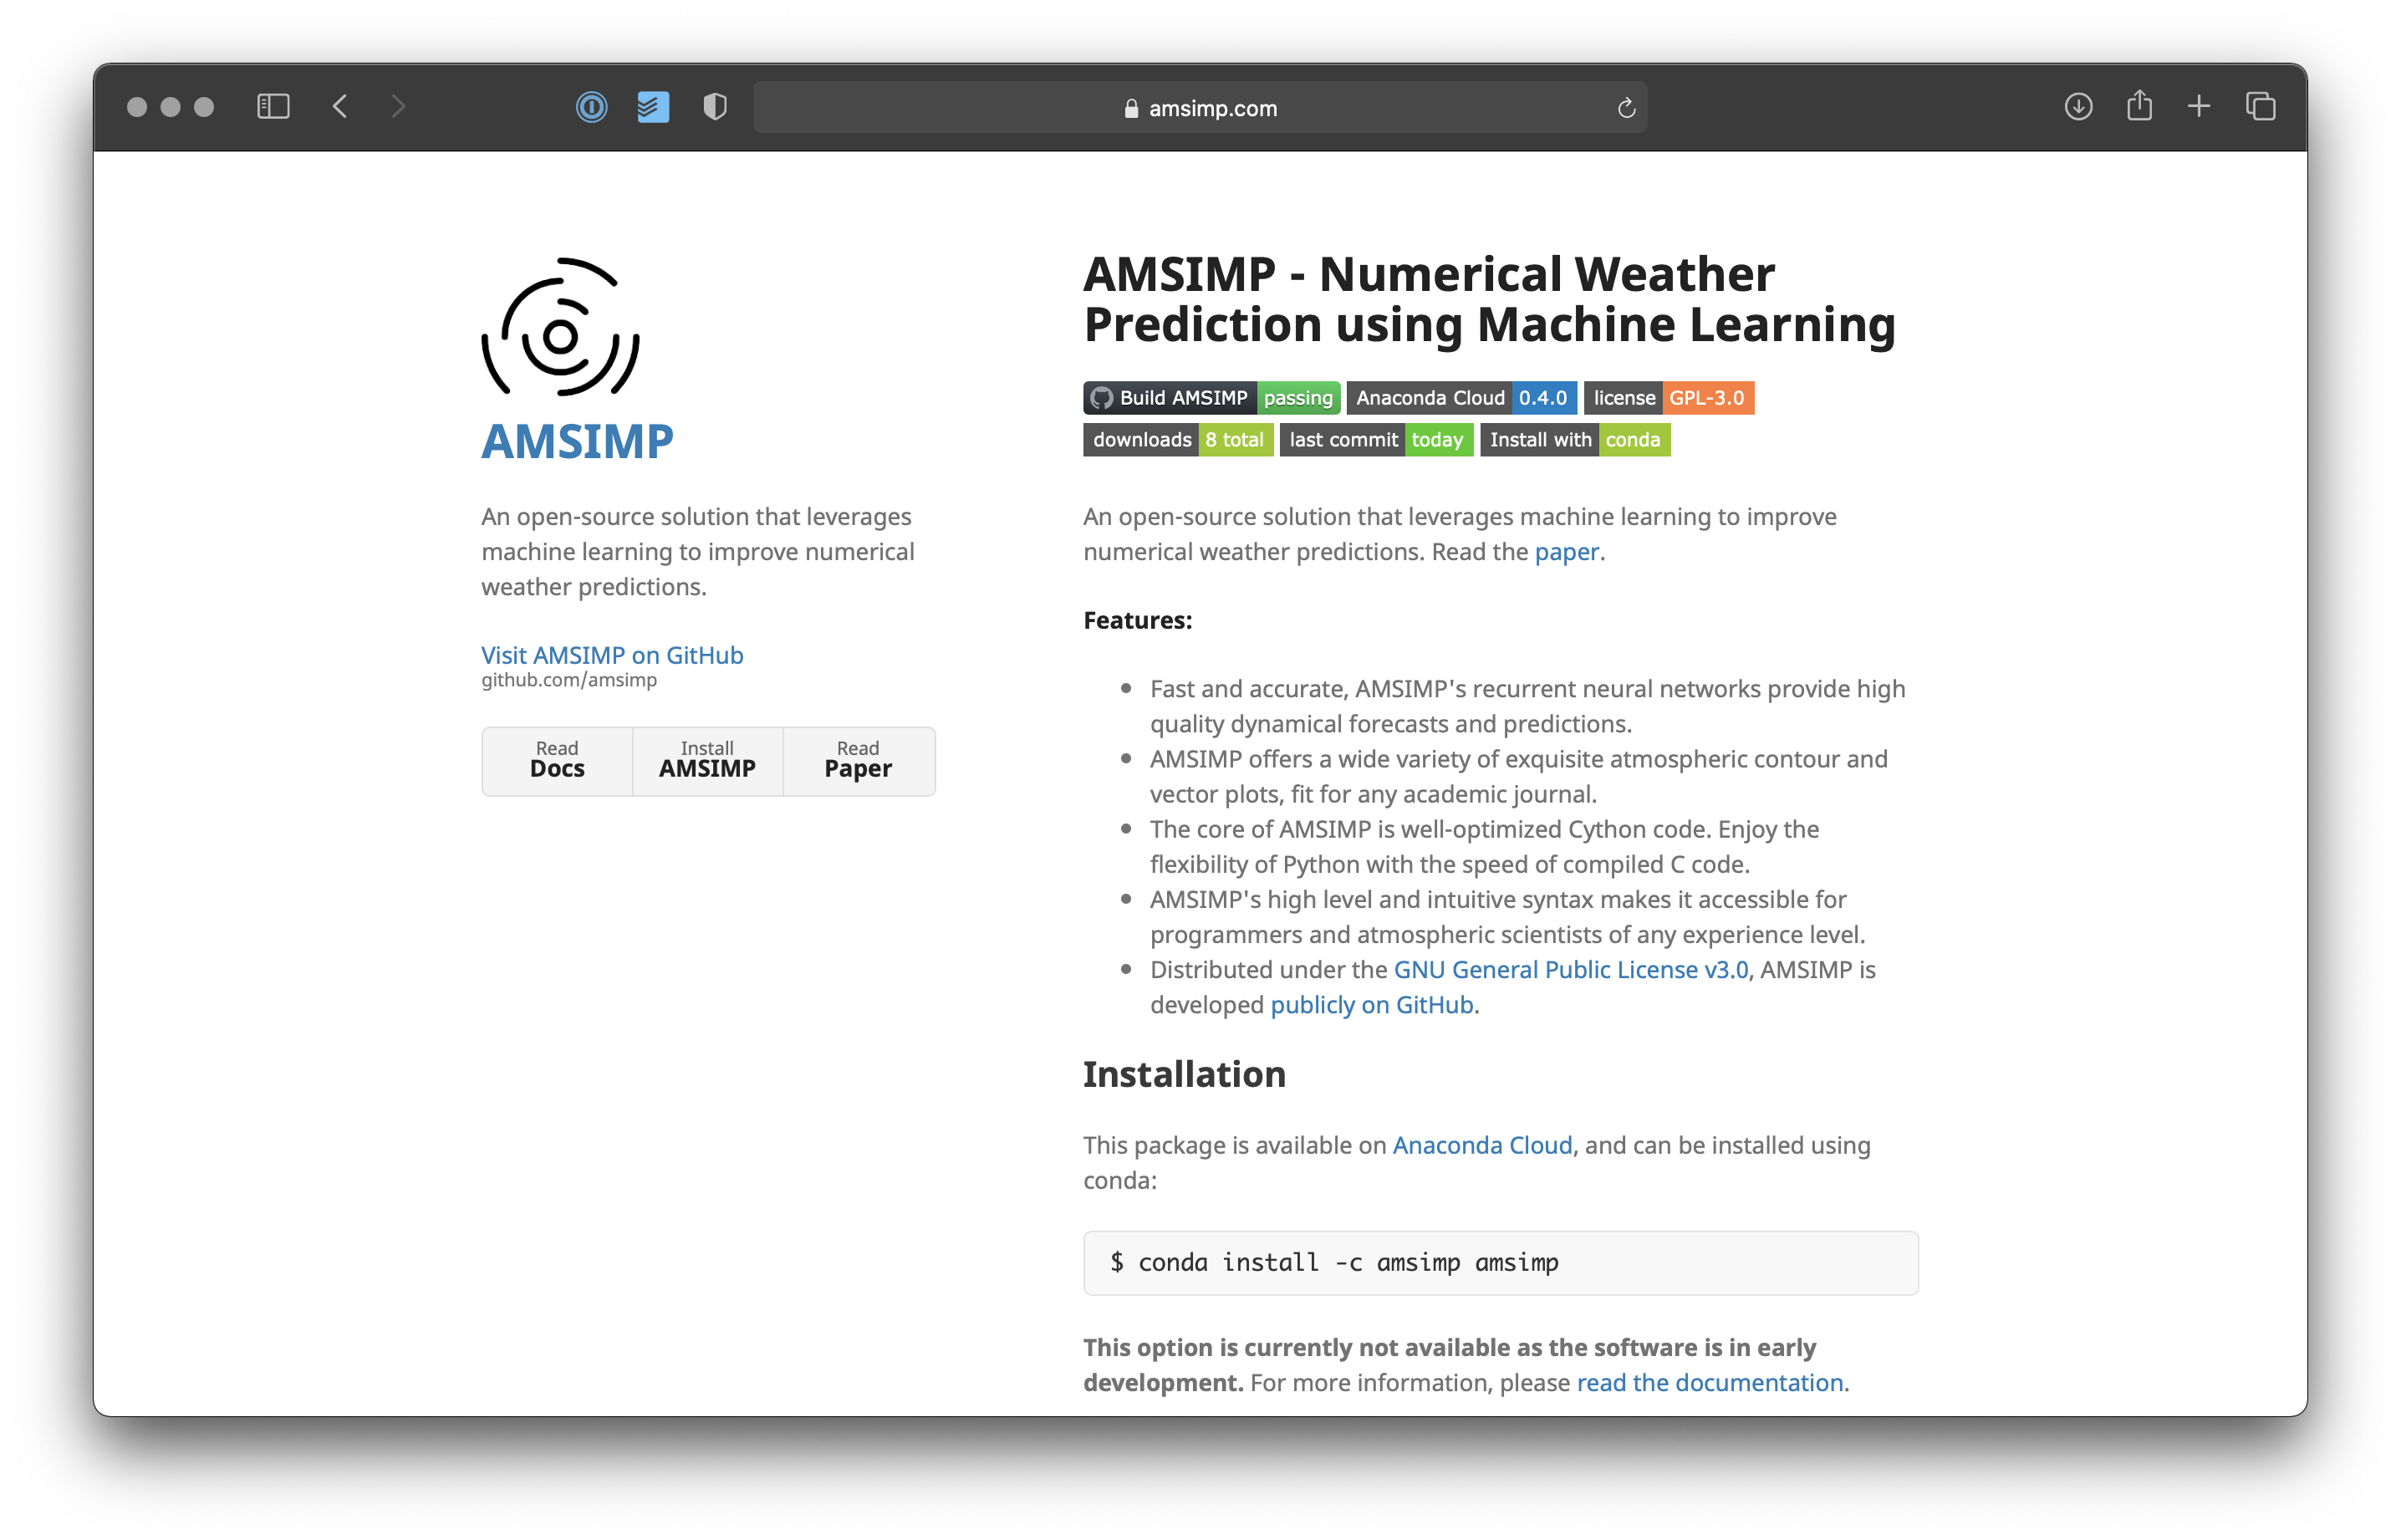
\includegraphics[width=.75\linewidth]{Images/website}
    \caption{A screenshot of the website for the software.}
    \label{website}
\end{figure}

\section{Organisation of this Work}
The work contained in this project book is broken down into a number of different chapters:

\begin{itemize}
    \item Chapter \ref{architecture_chapter} discusses the various neural network architecture under consideration and the current implementation within the software.
    \item Chapter \ref{implementation_chapter} discusses some of the decisions made on the software development side of the project, such as, choosing an appropriate programming language for the task. 
    \item Chapter \ref{benchmarking_chapter} outlines the software benchmarking experiments to be carried out on the software.
    \item Chapter \ref{results_chapter} contains the results of the benchmarking described in the previous chapter.
    \item Chapter \ref{conclusion_chapter} reviews the results and outcomes of the project, discusses the limitations of the software, and lays out a road-map for the continued development and enhancement of the software. 
\end{itemize}


\chapter{Model Architecture}\label{architecture_chapter}
\epigraph{``Since Newton, mankind has come to realise that the law of physics are always expressed in the language of differential equations"}{Steven Strogatz}

\section{RNN}
\subsection{Introduction}
Weather forecasting has traditionally been done by physical models of the atmosphere, which are unstable to perturbations, and thus are inaccurate for large periods of time\cite{why_rnn}. Since machine learning techniques are more sensitive to perturbations, it would be logical to combine a neural network with a physical model. Weather forecasting is a sequential data problem, therefore, a recurrent neural network is the most suitable option for this task. 

\begin{definition}
A recurrent neural network is a class of artificial neural networks where connections between nodes form a directed graph along a temporal sequence.
\end{definition}

Before, we delve into the specific example of using a recurrent neural network to predict the future state of the atmosphere, it is necessary to review what a recurrent neural network is. Recurrent Neural Networks (RNNs) are neural networks that are used in situations where data is presented in a sequence. For example, let's say you want to predict the future position of a fast-moving ball. Without information on the previous position of the ball, it is only possible to make an inaccurate guess. If you had, however, a large number of snapshots of the previous position, you are then able to predict the future position of the ball with some certainty. RNNs excel at modelling sequential data such as this. This is due to sequential memory.

In order to intuitively understand sequential memory, the prime example would be the alphabet. While it is easy to say the alphabet from A-Z, it is much harder to go from Z-A. There is a logical reason why this is difficult. As a child, you learn the alphabet in a sequence. Sequential memory is a mechanism that makes it easier for your brain to recognise sequence patterns.

In a traditional neural network, there is an input layer, hidden layer, and an output layer. In a recurrent neural network, a loop is added to pass information forward as seen in the diagram below (provided by Towards Data Science)\cite{intro_rnn}:

\begin{figure}[H]
    \centering
    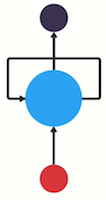
\includegraphics[width=.2\linewidth]{Images/rnn.png}
    \caption{Visualisation of a Recurrent Neural Network}
\end{figure}

The information that is forwarded is the hidden layer, which is a representation of previous inputs. How this works in practise is that you initialise your network layers and the initial hidden state. The shape and dimension of the hidden state will be dependent on the shape and dimension of your recurrent neural network. Then you loop through your inputs, pass the relevant parameter and hidden state into the RNN. The RNN returns the output and a modified hidden state. Last you pass the output of the hidden state to the output layer of the model, and it returns a prediction. 

There is, however, a major problem known as short-term memory. Short-term memory is caused by something known as the vanishing gradient problem, which is also prevalent in other neural network architectures. As the RNN processes more steps, it has troubles retaining information from previous steps. Short-Term memory and the vanishing gradient is due to the nature of back-propagation. This can be comprehended through understanding how a neural network is trained\cite{intro_rnn}.

\begin{definition}
Back-propagation is an algorithm used to train and optimise neural networks.
\end{definition}

To train a recurrent neural network, you use an application of back-propagation called back-propagation through time. Training a neural network has three major steps. First, the relevant data vector is normalised between 0 and 1, the vector is fed into the RNN, and it goes through an activation function. The activation function utilised in the software is the rectified linear activation function\cite{lstm_rnn}. 

\begin{definition}
The rectified linear activation function is a piece-wise linear function that will output the input directly if is positive, otherwise, it will output zero.
\end{definition}

The function is linear for values greater than zero, meaning it has a lot of the desirable properties of a linear activation function when training a neural network using back-propagation. Yet, it is a nonlinear function as negative values are always output as zero. As a result, the rectified function is linear for half of the input domain and nonlinear for the other half, it is referred to as a piece-wise linear function\cite{relu}. This nonlinear element is extremely important if the system has a nonlinear component, for example in predicting the evolution of the future state of the atmosphere.

\begin{figure}[H]
    \centering
    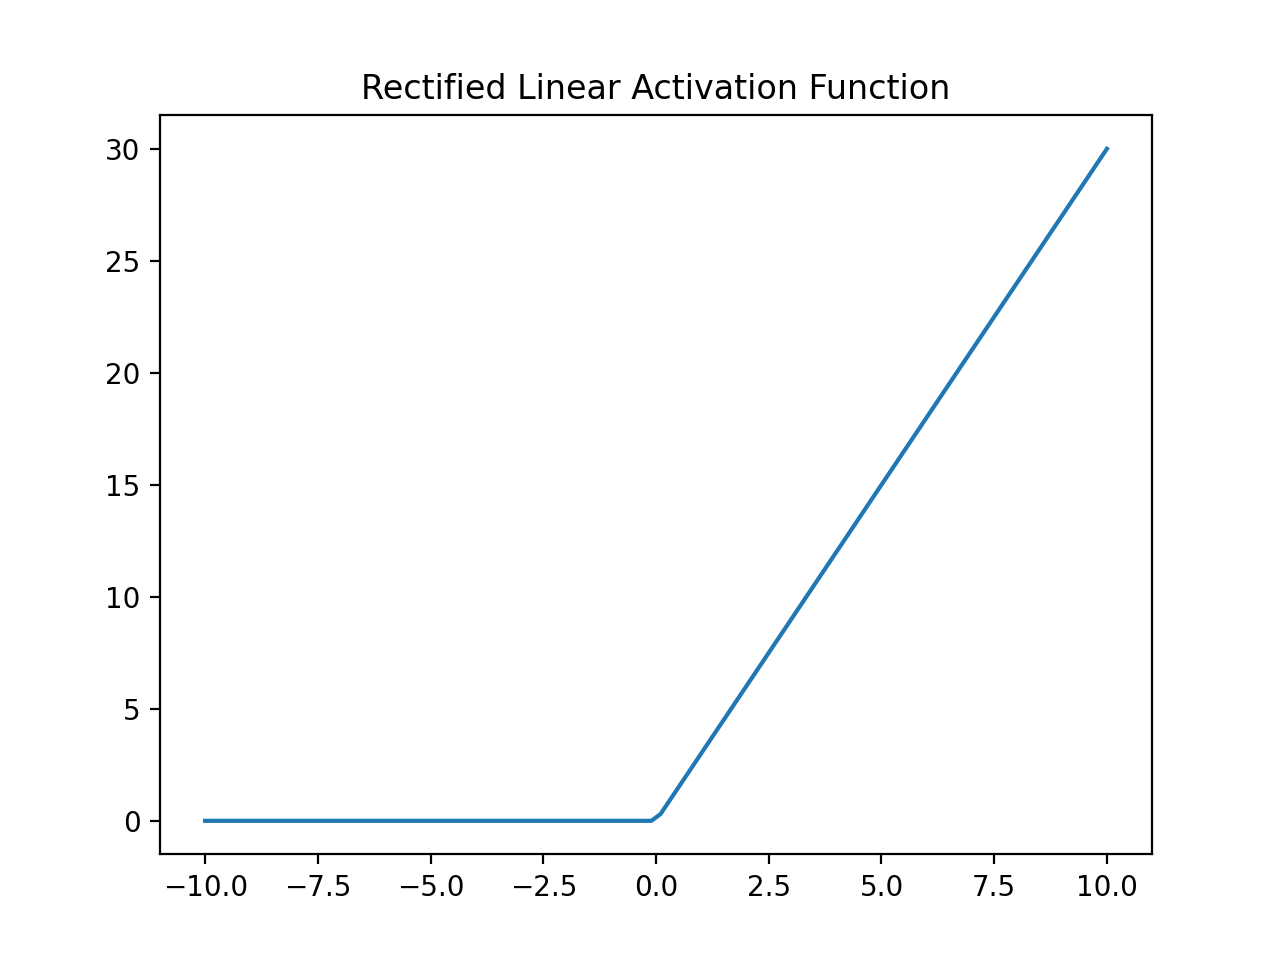
\includegraphics[width=.65\linewidth]{Images/relu.png}
    \caption{Sketch of the Rectified Linear Activation Function}
\end{figure}

Second, it outputs the results. Third, it compares the prediction to the observed state using a loss function.

\begin{definition}
A loss function outputs an error value which is an estimate of how poorly the network is performing.
\end{definition}

The lost function that will be utilised in the software will be the function for mean squared error. The reason for choosing this particular function is that it heavily penalises large errors, as it squares the difference between the predicted and actual value. A large error in a weather forecast is highly undesirable, hence, the use of this function. The function is represented below:

\begin{equation}
    MSE = \frac{1}{n}\sum_{i=1}^n(Y_i-\hat{Y_i})^2
\end{equation}

If  a vector of $n$ predictions is generated from a sample of $n$ data points on all variables, and $Y$ is the vector of observed values of the variable being predicted, with $\hat{Y_i}$ being the predicted values.

\begin{definition}
Mean squared error is the average squared difference between the estimated values and the actual value.
\end{definition}

Returning to the training of the RNN, it uses that error value from the loss function to do back propagation which calculates the gradients for each time step in the network. The gradient is the value used to adjust the networks internal weights, allowing the network to learn. The bigger the gradient, the bigger the adjustments and vice versa. Here is where the problem lies. When doing back propagation, the gradient of the current time step is calculated with respect to the effects of the gradients, in the time step before it. So if the adjustments to the time step before it is small, then adjustments to the current time step will be even smaller.  The gradient values will exponentially shrink as it propagates through each time step. That causes gradients to exponentially shrink as it back propagates down. The earlier layers fail to do any learning as the internal weights are barely being adjusted due to extremely small gradients.

Because of vanishing gradients, the RNN doesn’t learn the long-range dependencies across time steps. So not being able to learn on earlier time steps causes the network to have a short-term memory. In order to combat this, a long short-term memory is used\cite{intro_rnn}.

\subsection{LSTM}
LSTM's were created as a solution to the short-term memory problem. They have internal mechanisms called gates that can regulate the flow of information. These gates can learn which data in a sequence is important to keep or throw away. By doing that, it can pass relevant information down the long chain of sequences to make predictions. For example, if you were interested in buying a particular product, you might read a review in order to determine if the purchase of the product is a good decision. When you read a review, your brain subconsciously only remembers important keywords. You pick up words like ``amazing", ``superb", or ``awful", you don't remember words such as "the", "as", or "because". This is what an LSTM does, it learns to keep only the relevant information to make predictions.

An LSTM has a similar control flow as a recurrent neural network. It processes data passing on information as it propagates forward. The differences are the operations within the LSTM’s cells. The core concept of LSTM’s are the cell state, and it’s various gates. The cell state is the method by which information is transferred down the sequence chain. The cell state, in theory, can carry relevant information throughout the processing of the sequence. So even information from the earlier time steps can make its way to later time steps, reducing the effects of short-term memory. As the cell state goes on its journey, information gets added or removed to the cell state via gates\cite{lstm_rnn}.

\begin{definition}
A gate is an electric circuit with an output which depends on the combination of several inputs.
\end{definition}

Gates contain the sigmoid activation function. The sigmoid activation function squishes values between 0 and 1. That is helpful to update or forget data because any number getting multiplied by 0 is 0, causing values to disappears or be ``forgotten". Any number multiplied by 1 is the same value therefore that value stays the same or is ``kept".

\begin{figure}[H]
    \centering
    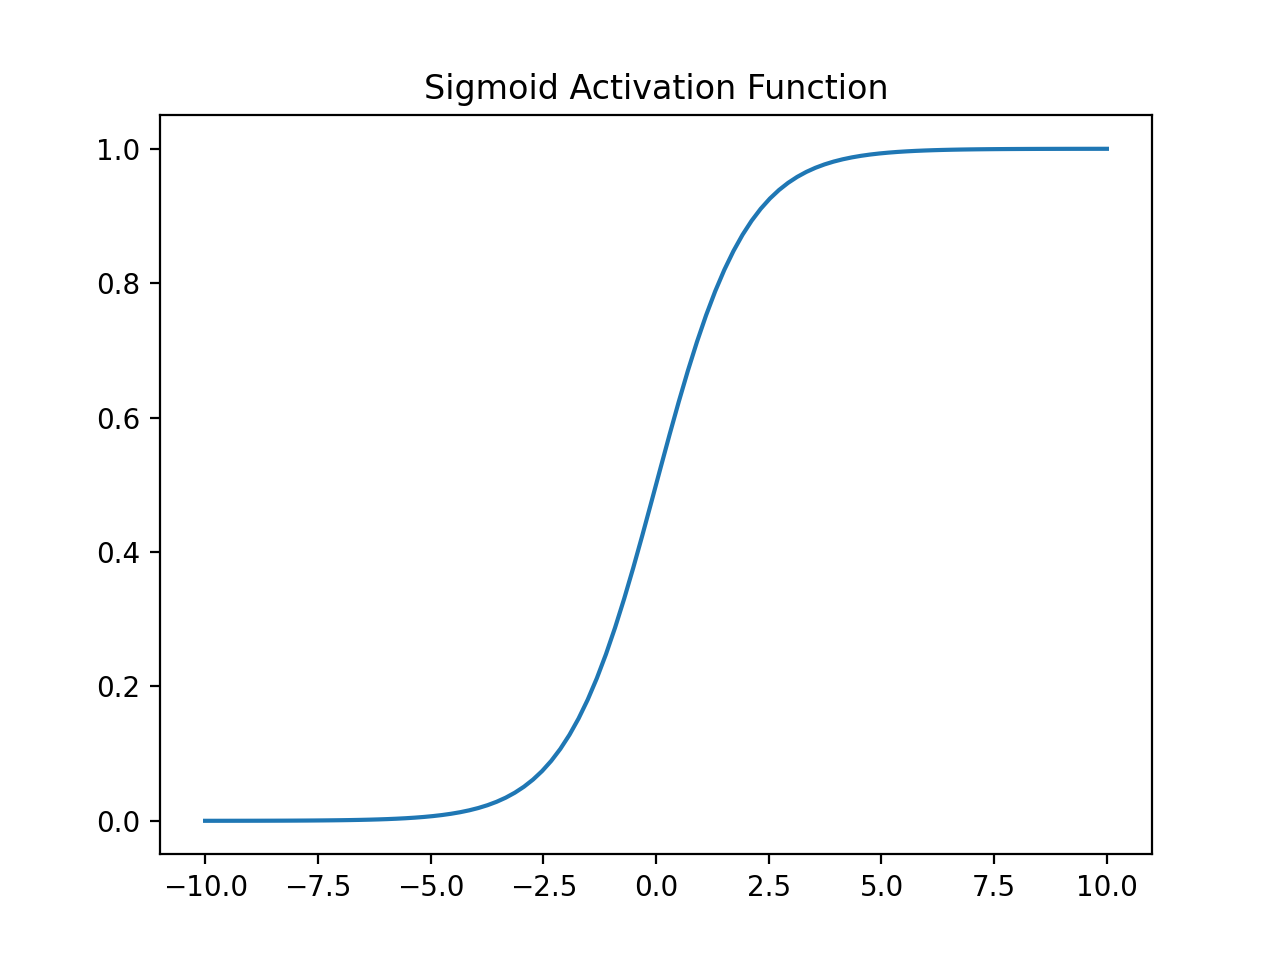
\includegraphics[width=.65\linewidth]{Images/sigmoid.png}
    \caption{Sketch of the Sigmoid Activation Function}
\end{figure}

There are three types of gates utilised within a neural network: a forget gate, an input gate, and an output gate. A forget gate decides what information should be thrown away or kept. Information from the previous hidden state and information from the current input is passed through the sigmoid function. An input gate is where the previous hidden state and current input are passed into a sigmoid function. The output gate decides what the next hidden state should be. The hidden state is also used for predictions. First, we pass the previous hidden state and the current input into a sigmoid function. Then we pass the newly modified cell state to the rectified linear activation function. We multiply the rectified linear activation function output with the sigmoid output to decide what information the hidden state should carry. The output is the hidden state. The new cell state and the new hidden state is then carried over to the next time step\cite{lstm_rnn}.

\subsection{Convolutional LSTM Network}
The formulation of a numerical weather prediction model is a spatiotemporal sequence forecasting problem that can be solved under a general sequence-to-sequence learning framework. 

\begin{definition}
A spatiotemporal sequence is a sequence that contains both spatial and temporal information.
\end{definition}

In order to better model the spatiotemporal relationships, this project will utilise ConvLSTM layers; which was proposed by Xingjian Shi et. al\cite{convlstm}. This spatiotemporal sequence forecasting problem is different from the one-step time series forecasting problem because the prediction target of the problem is a sequence which contains both spatial and temporal structures. Although a LSTM layer has proven powerful for handling temporal correlation, it contains too much redundancy for spatial data. To address this problem, this project will use a ConvLSTM layer which has convolutional structures in both the input-to-state and state-to-state transitions\cite{convlstm}.

The major drawback of LSTMs is in the handling spatiotemporal data due to its usage of full connections in input-to-state and state-to-state transitions in which no spatial information is encoded. To overcome this problem, a distinguishing feature of a ConvLSTM cell is that all the inputs and gates of the ConvLSTM layer are 3D tensors whose last two dimensions are spatial dimensions. To get a better picture of the inputs and states, we may imagine them as vectors standing on a spatial grid. The ConvLSTM determines the future state of a certain cell in the grid by the inputs and past states of its local neighbour. This can easily be achieved by using a convolution operator in the state-to-state and input-to-state transitions\cite{convlstm}. This is what the ConvLSTM layer does.

\begin{figure}[H]
    \centering
    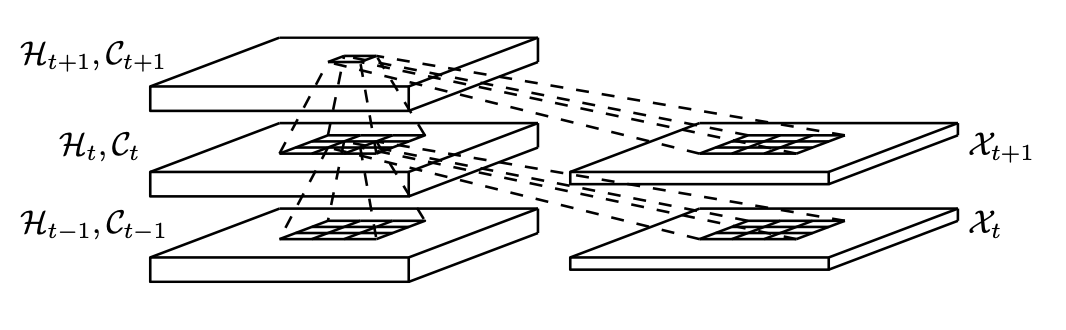
\includegraphics[width=.8\linewidth]{Images/convlstm.png}
    \caption{The architecture of a ConvLSTM cell.}
\end{figure}

\section{Dataset}
\subsection{ERA5 Atmospheric Reanalysis Dataset}\label{era5_dataset}
ERA5 provides hourly estimates of a large number of atmospheric, land and oceanic climate variables. The data covers the Earth on a 30km grid and resolves the atmosphere using 137 levels from the surface up to a height of 80km. ERA5 includes information about uncertainties for all variables at reduced spatial and temporal resolutions. Quality-assured monthly updates of ERA5 are published within 3 months of real time. Preliminary daily updates of the dataset are available to users within 5 days of real time. ERA5 combines vast amounts of historical observations into global estimates using advanced modelling and data assimilation systems\cite{era5}.

The ERA5 reanalysis dataset was used for training, validating and testing the performance of the neural network architecture. Reanalysis datasets provide the best guess of the atmospheric state at any point in time by combining a forecast model with the available observations. The raw data is available hourly for 40 years from 1979 to 2019 on a $0.25^{\circ}$ latitude-longitude grid ($721 \times 1440$ grid points) with 37 vertical levels. Since this raw dataset is quite significant, it is necessary to regrid the dataset to a lower resolution and use a smaller fraction of the available dataset\cite{rasp2020weatherbench}.  The poles were excluded from the dataset in order to avoid a singularity, and the potential negative impact that could have on predictive ability of the neural network.

It was ultimately decided to use a spatial resolution of $1^{\circ}$ ($179 \times 360$ grid points) and a temporal resolution of 2 hours. The data is split into yearly NetCDF files for each variable. The entire dataset at $0.25^{\circ}$ resolution has a size of 400GB, before the dataset was interpolated to a grid of a lower resolution. The prognostic variables of interest are temperature and geopotential, and were chosen based on meteorological considerations. Geopotential, and temperature are prognostic state variables in most physical numerical weather prediction and climate models\cite{rasp2020weatherbench}. 

\subsection{Integrated Forecasting System}\label{ifs_section}
The Integrated Forecast System is a global numerical weather prediction system developed and maintained by the European Centre for Medium-Range Weather Forecasts organisation. The version of the IFS run at ECMWF is often referred to as the ``ECMWF" or the ``European model" in North America, to distinguish it from the American GFS. It comprises of a spectral atmospheric model with a terrain-following vertical coordinate system coupled to a 4D variational data assimilation system. In 1997 the IFS became the first operational forecasting system to use a 4D variational, data assimilation system

\begin{definition}
4D dimensional variational data assimilation system adjusts a short-range forecast, called the background, in space and time to bring it into closer agreement with meteorological observations.
\end{definition}

\begin{figure}[H]
    \centering
    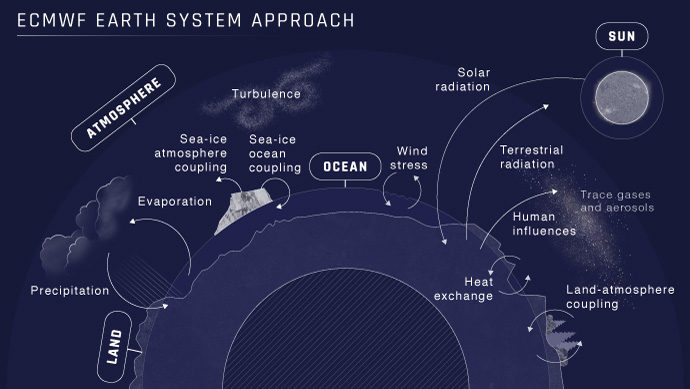
\includegraphics[width=.8\linewidth]{Images/ifs.jpg}
    \caption{ECMWF Integrated Forecast System}
\end{figure}

It is one of the predominant global medium-range models in general use worldwide; its most prominent rival in the 6–10 day medium range include the American Global Forecast System, the Canadian Global Environmental Multiscale Model and the UK Met Office Unified Model. For context, Met Éireann utilises the IFS for medium-range forecasts; however for short-range forecasts, Met Éireann uses its own HARMONIE-AROME NWP model. The operational configuration consists of $1000 \times 900$ grid points in the horizontal at 2.5km resolution, with 65 levels in the vertical. A 54-hour forecast is produced four times a day, at 00Z, 06Z, 12Z and 18Z\cite{harmonie_arome_nwp}. 

The IFS is the gold standard of medium-range numerical weather prediction. The current IFS deterministic forecast is computed on a cluster with 11,664 cores. One 10 day forecast at 10 km resolution takes around 1 hour of real time to compute\cite{rasp2020weatherbench}. The Integrated Forecasting System will be used as a comparison against the neural network.

To provide physical baselines more in line with the current resolution of the neural network, it was compared against the IFS model at two coarser horizontal resolutions, T42 (approximately $2.8^{\circ}$) with 62 vertical levels and T63 (approximately $1.9^{\circ}$) with 137 vertical levels. It must be noted that I personally did not generate such forecasts, or perform the analysis on said forecasts. It acquired the results from Weather Bench, a benchmark dataset for data-driven weather forecasting. According to said source; computationally, a single forecast takes 270 seconds for the T42 model and 503 seconds for the T64 model on a single XC40 node with 36 cores.

\section{Implementation}\label{implement_rnn}
Drawing from knowledge of current numerical weather prediction model frameworks, it may seem intuitive to train a machine learning model to produce the best possible single‐step forecast from a given atmospheric state. In practice, this can yield a model that performs well for short‐range forecasts but diverges from reality for longer range predictions. This is because there are no constraints on the CNN, physical or mathematical, that would prevent it from diverging from reality when its prediction fed back in as inputs no longer resemble an atmospheric state in the training data. In order to nudge the numerical weather prediction model toward learning to predict longer‐term weather and improve its long‐term stability, the model will be trained on multiple iterated predictive steps. 

Initially, the model inputs included two time steps and it is tasked with predicting two output time steps. This resulted in the first couple of time step predictions producing relatively decent result, however, it quickly diverged from reality after this point. Hence, it was necessary to increase both the time steps and the output time steps to six. This increased the overall numerical stability of the model. 

The dataset consists of three features: air temperature at a pressure surface of 850 hPa, geopotential at a pressure surface of 500 hPa, and air temperature at 2 metres above the surface. For a single day, there is twelve observations. The goal for this project will be to predict the relevant atmospheric parameter in 12 hours time given the last twelve hours of data. In order to make such predictions, it is necessary to create a window of the last 6 ($\frac{12}{2}$) observations to train the model\cite{time_series}. The neural network was trained on observational data from 2009 to 2015. The remainder of the dataset, 2016 to 2019, was preserved for validation, testing and benchmarking the neural network against physics-based models. The model was built using the open‐source Keras library for Python with Google's TensorFlow backend\cite{numerical_stability}.

\begin{minted}[mathescape,linenos,frame=lines]{python}
# Optimiser.
opt = Adam(lr=1e-3, decay=1e-5)
\end{minted}

Adam optimisation was chosen as the most appropriate optimiser for this particular model. This is a stochastic gradient descent method that is based on adaptive estimation of first-order and second-order moments. This method is computationally efficient, has little memory requirements, invariant to diagonal rescaling of gradients, and is well suited for problems that are large in terms of parameters.

\begin{minted}[mathescape,linenos,frame=lines]{python}
# First layer of model.
model.add(
    ConvLSTM2D(
        filters=64, 
        kernel_size=(7, 7),
        input_shape=(6, 179, 360, 3), 
        padding='same', 
        return_sequences=True, 
        activation='tanh', 
        recurrent_activation='hard_sigmoid',
        kernel_initializer='glorot_uniform', 
        unit_forget_bias=True, 
        dropout=0.3, 
        recurrent_dropout=0.3, 
        go_backwards=True
    )
)
\end{minted}

The above code is the first layer of the model. The activation functions utilised in this layer are predefined within Tensorflow, and have been described at great length previously. The model consists of four ConvLSTM layers in total, with similar parameters as the aforementioned layer with a few variations.

\begin{minted}[mathescape,linenos,frame=lines]{python}
# Batch normalisation.
model.add(BatchNormalization())
\end{minted}

A consistent challenge in machine learning is that the model is updated layer-by-layer backward from the output to the input using an estimate of error that assumes the weights in the layers prior to the current layer are fixed. Because all layers are changed during an update, the update procedure is forever chasing a moving target. A batch normalisation layer occurs after each ConvLSTM layer to resolve this problem.  

\begin{definition}
Batch normalization is a technique to help coordinate the update of multiple layers in the model.
\end{definition}

It does this by scaling the output of the layer, specifically by standardising the activation of each input variable per mini-batch, such as the activation of a node from the previous layer. Standardising the activation of the prior layer means that assumptions the subsequent layer makes about the spread and distribution of inputs during the weight update will not change. This has the effect of stabilising and speeding-up the training process of neural networks\cite{batch_normalization}.

\begin{minted}[mathescape,linenos,frame=lines]{python}
# Dropout.
model.add(Dropout(0.1))
\end{minted}

Each batch normalisation layer is then followed by a dropout. Dropout is a regularisation method that approximates training a large number of neural networks with different architectures in parallel. During training, some number of layer outputs are randomly ignored or “dropped out.” This has the effect of making the layer look-like and be treated-like a layer with a different number of nodes and connectivity to the prior layer. In effect, each update to a layer during training is performed with a different “view” of the configured layer. Dropout has the effect of making the training process noisy, forcing nodes within a layer to probabilistically take on more or less responsibility for the inputs. This conceptualisation suggests that perhaps dropout breaks-up situations where network layers co-adapt to correct mistakes from prior layers, in turn making the model more robust\cite{dropout}.

\begin{minted}[mathescape,linenos,frame=lines]{python}
# Add dense layer.
model.add(Dense(3))
\end{minted}

Following the final ConvLSTM layer, a dense layer is implemented. The dense layer is a neural network layer that is connected deeply, which means each neuron in the dense layer receives input from all neurons of its previous layer\cite{dense}. In our case, it results in the model outputting the expected shape by reducing the filters down to the three previously mentioned features. The code for the model in its entirety can be found in appendix \ref{model_code}. 


\chapter{Implementation Details}\label{implementation_chapter}
\epigraph{``Curious that we spend more time congratulating people who have succeeded than encouraging people who have not."}{Neil deGrasse Tyson}

\section{Open Source Software}
As mentioned previously, and to the author's knowledge, there is no open source software currently available that can numerically simulate the dynamics of the atmosphere. But, what is open source software, what are its advantages, and why is it important?

\begin{definition}
Open Source Software is software with source code that anyone can inspect, modify, and enhance. 
\end{definition}

Source code is the code that computer programmers use to modify, and change how a piece of software functions\cite{what_oss}. Programmers with access to the source code can improve that program by adding features to it, fixing bugs, or by improving the documentation of the surrounding source code. 

According to Tom Macaulay\cite{advantages}, the open source development of software has a number of advantages over the traditional development of proprietary software, including but not limited to:

\begin{itemize}
    \item Lower costs.
    \item Extensive customisation.
    \item Higher quality software.
    \item Greater security.
    \item Regular updates.
    \item Quick fixes.
\end{itemize}

If an atmospheric dynamics simulator became available to the open source community, it could lead to a low cost, and high quality simulator ultimately being produced. If such an event occurs, it could, theoretically, vastly enhance existing weather predicting software, and could lead to a further dramatic decline in deaths from weather related phenomena. This project is an attempt to kick start such a future.

Everything related to this project, from the source code of the simulator to this very paper, can be accessed at the organisation known as `AMSIMP' on the open source platform known as GitHub. This can be accessed at \url{https://github.com/amsimp}. 

\begin{figure}[H]
    \centering
    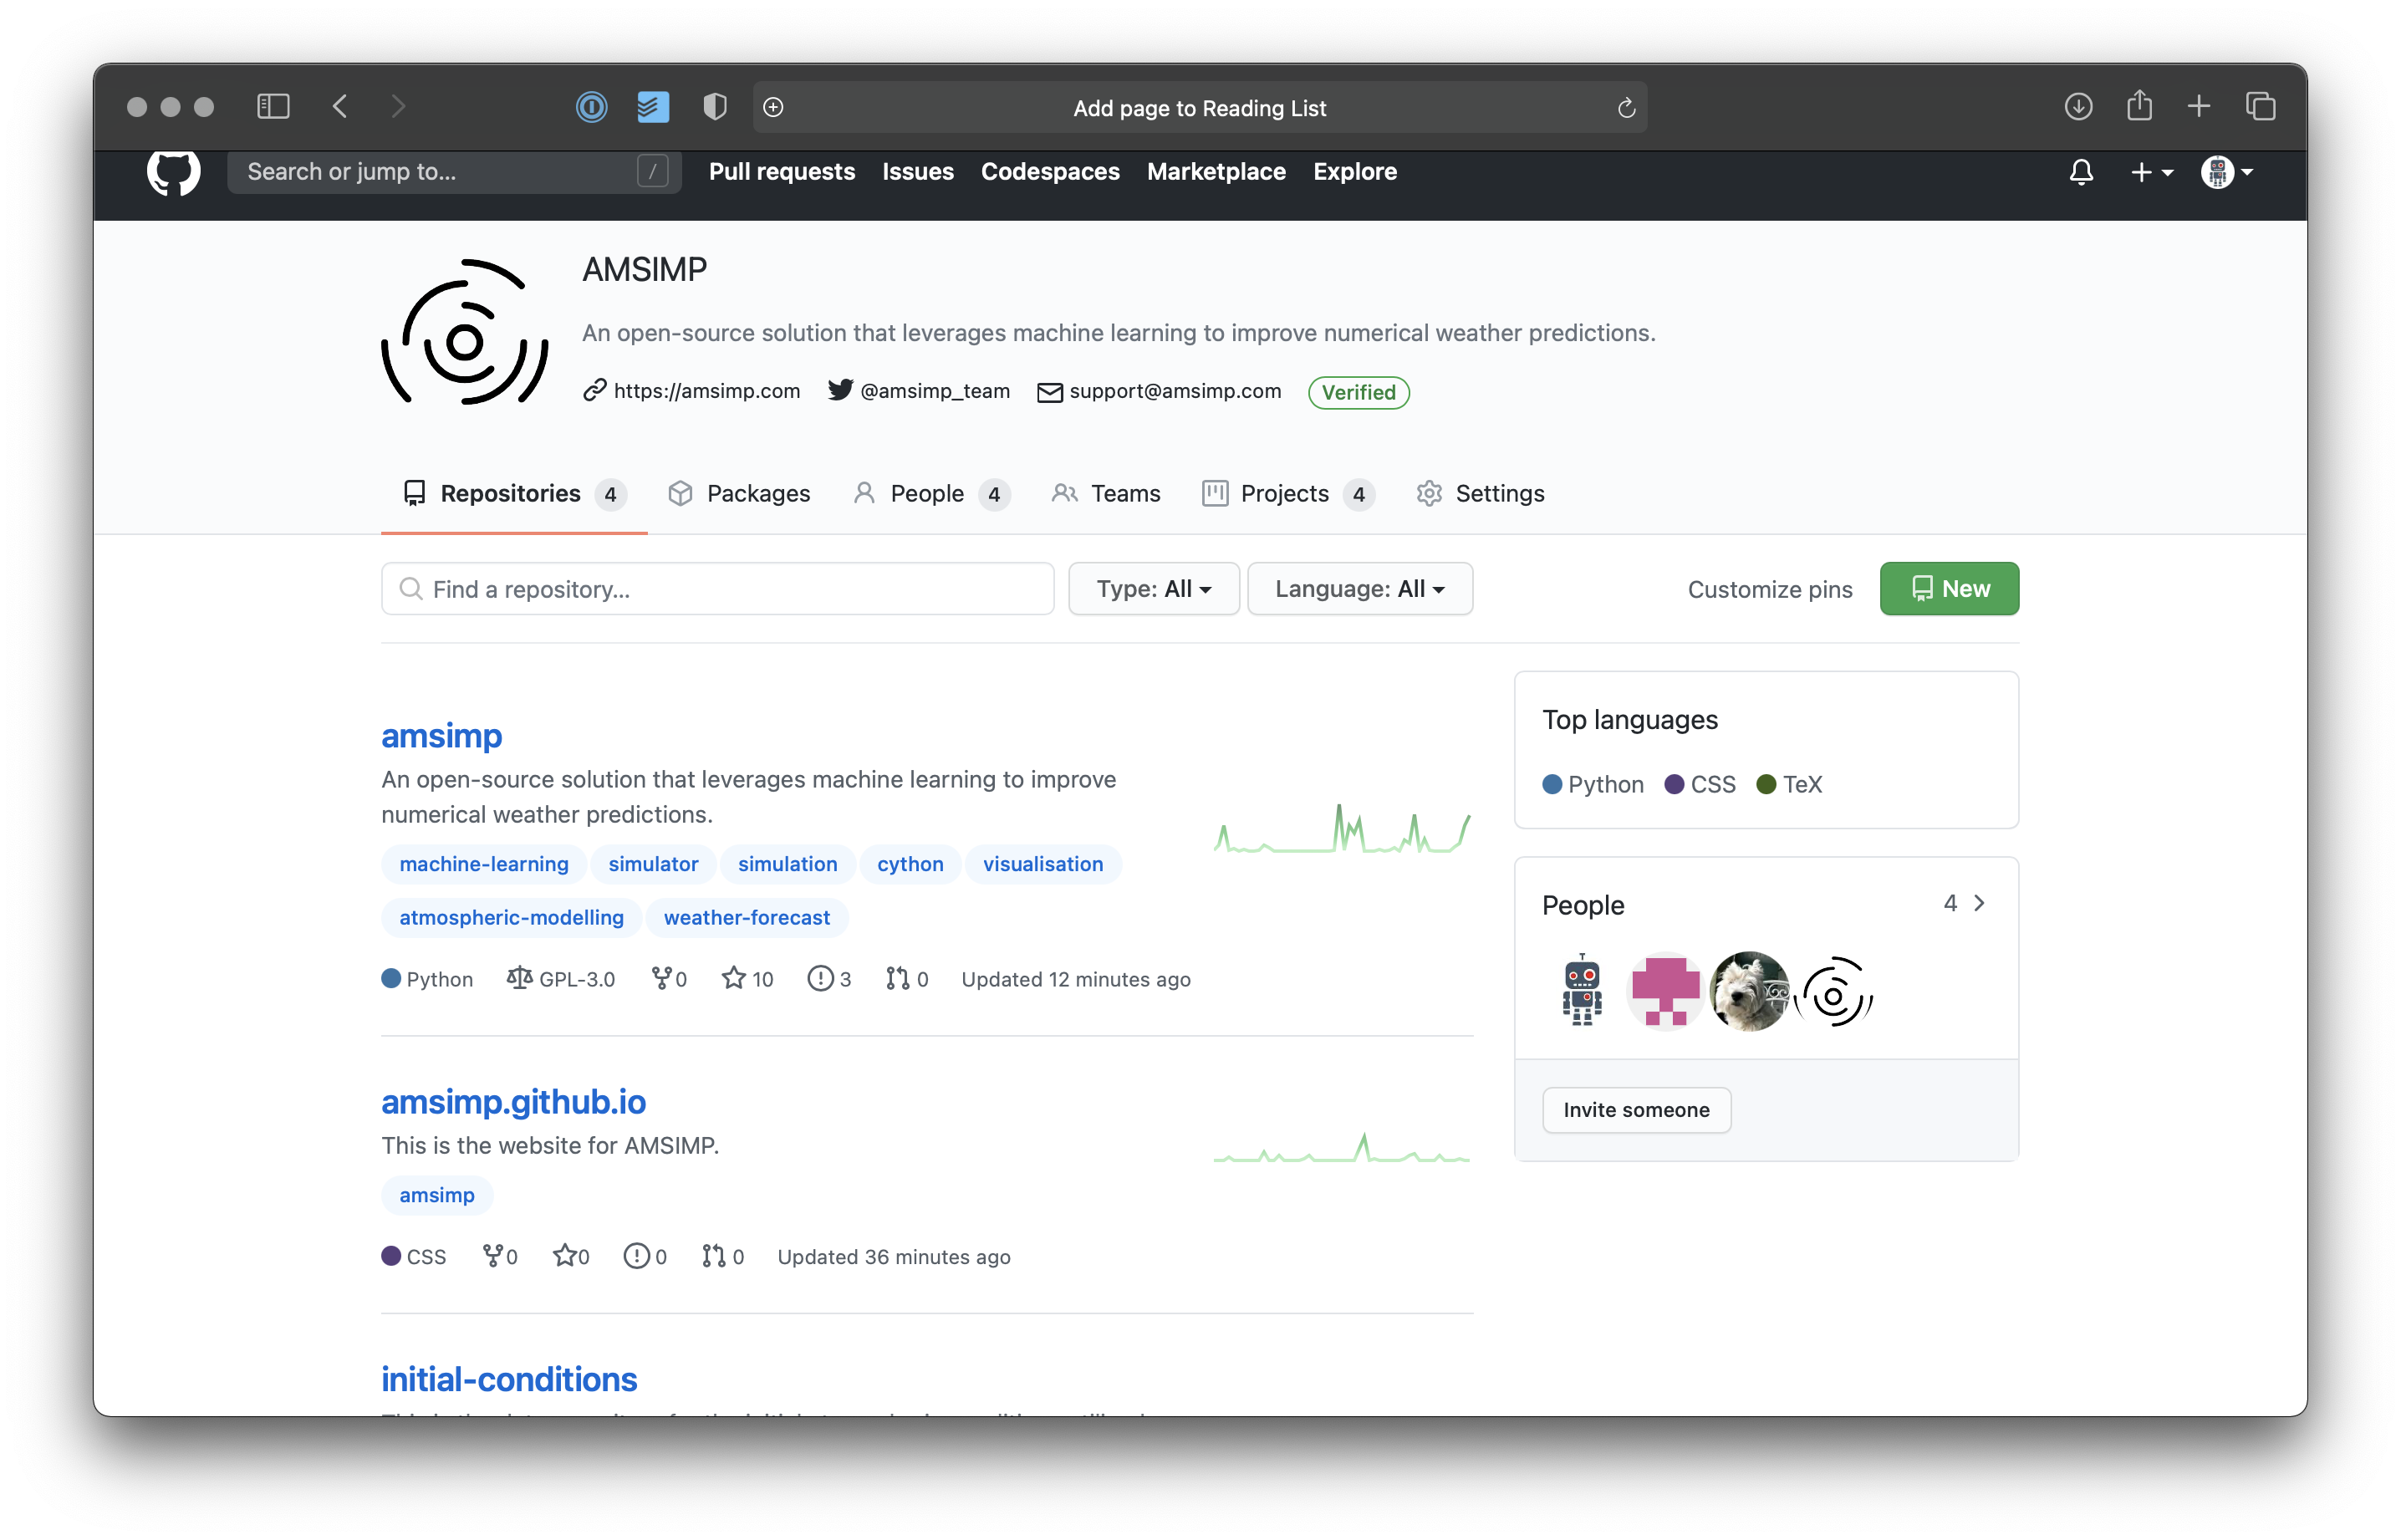
\includegraphics[width=.8\linewidth]{Images/github}
    \caption{A screenshot of the AMSIMP organisation, hosted by the open source platform known as GitHub.}
    \label{github}
\end{figure}

\section{Language Selection}
\subsection{Initial Language Selection}
The most crucial element of this project was choosing an appropriate programming language for the task. During the initial consideration period, I analysed two different programming languages: JavaScript, and Python\cite{python}. 

Initially, I considered the programming language, JavaScript with a run-time environment known as Node.js (Node.js executes code outside of a browser), for two reasons primarily:

\begin{itemize}
    \item JavaScript excels at data visualisation.
    \item Node.js is extremely well suited for memory intensive activities.
\end{itemize}

In line with the expectation of using this programming language, Miss Abbott, and I attended the Dublin Node.js Meetup on the 28th of February. I did this in order to gain an understanding of what Node.js is used for, and what would be the best way one would go about using it. 

In the end, however, I ultimately chose Python for the task due to a number of shortcomings on the part of JavaScript (Node.js), and advantages on the part of Python. Firstly, JavaScript just doesn’t have the same enormous suite of scientific packages and inbuilt functionality that Python does. Using JavaScript, therefore, would waste valuable development time, and ultimately would be entirely inefficient.

Secondly, Python already has an extensive ecosystem with how-to’s available for almost any scientific task you would ever want to do. For JavaScript, this is simply not the case.\cite{javascript_vs_python}

\subsection{Switching to Cython}
During the continued development of the software over the summer months, I discovered a rather severe bottleneck as a result of my choice of programming language: the execution time performance. The culprit behind this bottleneck was a result of Python's dynamically typed nature. Generally, you can classify programming languages into two categories: dynamically typed languages and statically typed languages. 

\begin{definition}
A dynamically typed language is one in which the type of the variable is not known at compile time, and generally, you can define a variable as an integer type at the start of the program for example and later redefine it as a string type. 
\end{definition}

On the other hand, a statically typed language is a language where the type of variable is known at compile time, and during the execution of the program, the variable type must remain constant. 

\hfill

\begin{figure}[H]
    \centering
    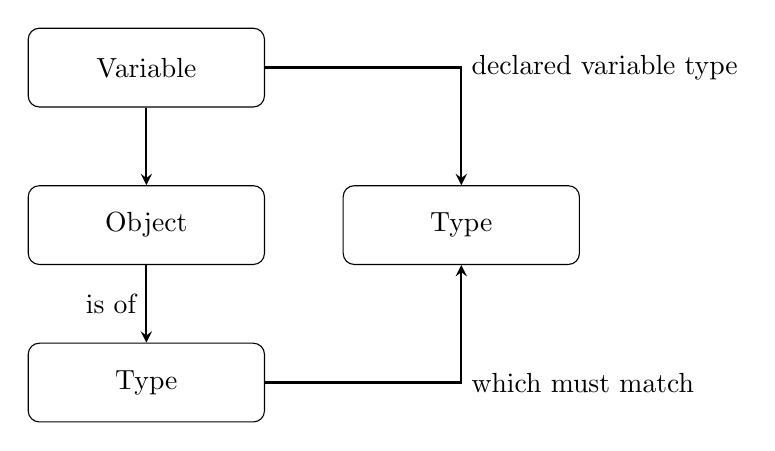
\begin{tikzpicture}[node distance=2cm]
        \tikzstyle{startstop} = [rectangle, rounded corners, minimum width=3cm, minimum height=1cm,text centered, draw=black]
        \tikzstyle{arrow} = [thick,->,>=stealth]
        
        \node (start) [startstop] {Variable};
        \node (obj) [startstop, below of=start] {Object};
        \node (type1) [startstop, right of=obj, xshift=2cm] {Type};
        \node (type2) [startstop, below of=obj] {Type};
        
        \draw [arrow] (start) -- (obj);
        \draw [arrow] (start) -| node[anchor=west] {declared variable type} (type1);
        \draw [arrow] (obj) -- node[anchor=east] {is of} (type2);
        \draw [arrow] (type2) -| node[anchor=west] {which must match} (type1);
    \end{tikzpicture}
    \caption{How statically typed languages handle variables.}
\end{figure}

A statically typed language is particularly useful for software with a large number of loops, or repetitive calculations contained within them. During a loop, a dynamically typed language will continuously check the type of variable after each loop, even if it has done so in previous loops. In a small number of loops, this has a negligible impact on the execution time; however, in a large enough quantity, this has a cumulative effect, significantly stifling the execution time performance. Generally, a piece of software written in a statically typed language will execute a lot faster; this fact will be demonstrated in chapter \ref{6}. The reason behind picking Cython over other statically typed languages, such as C, is that Cython retains all the benefits of Python, with its extensive scientific package library and its simple syntax, while gaining the performance benefits of a statically typed language.



\chapter{Benchmarking}\label{benchmarking_chapter}
\epigraph{``It's known in theory that log(log(n)) approaches infinity, but no one has ever observed it in practice."}{Grant Sanderson}

To prove the hypothesis that `it is possible to create open source software implementation to simulating atmospheric dynamics, with a recurrent neural network and ensemble prediction system being used in combination with a physical model, that such a software implementation has a reasonable execution time to forecast length ratio, and to determine if such an implementation has a statistically significant accuracy improvement over a traditional deterministic physical model', it is necessary to carry out a series of appropriate benchmarks.

It was determined that it was necessary to carry out a series of appropriate benchmarking within the areas of performance, and accuracy. The performance benchmark would demonstrate whether or not the software has a reasonable execution time to forecast length ratio, and the accuracy benchmark would highlight whether or not the forecasts produced by the software had a reasonable level of accuracy. Considering there is no open source software to which one can compare the software, it was determined that the software would be compared against a proprietary implementation. For this purpose, OpenWeatherAPI was selected as the most appropriate option as it provides accurate data for slightly longer time ranges than other similar application programming interfaces\cite{owa}. 

Please note that all of the benchmarking code is available on the AMSIMP repository, which can be accessed using the following url: \url{https://github.com/amsimp/initial-conditions}

\section{Performance Benchmark}
One of the most important factors to consider when benchmarking a piece of software is the execution time of said software. A piece of software can be as precise and accurate as it wants, however, it isn't of much practical use if it takes the length of time until the heat death of the universe to finish executing. For example, attempting to brute force a 12 character alphanumeric password might work, however, it would take approximately two centuries based on the current capabilities of computers. Considering simulating atmospheric dynamics requires a significant amount of computational resources, it was deemed necessary to run the software on a virtual machine. Using a virtual machine also allows for easier replication and duplication of results, especially considering the wide variety of computer hardware available today. Google's Compute Engine was ultimately chosen as it provided the most flexibility, with the amount of promotional credit being significantly greater than the competition. Without the promotional credit, the benchmarking process would have been an extremely expensive affair to complete (the hardware specification below would have cost approximately one dollar an hour). It was also deemed the only feasible option available due to the restrictions imposed by the COVID-19 pandemic. 

\subsection{Hardware Specifications}\label{specs}
\begin{center}
\begin{tabular}{|c|c|} 
 \hline
  & Compute Engine n1-custom-configuration \\
 \hline
 \textbf{vCPUs} & 8 \\
 \hline
 \textbf{Memory} & 128 GB \\
 \hline
 \textbf{Operating System} & Ubuntu 20.04 LTS \\
 \hline
\end{tabular}\par
\bigskip
Table 5.3.: Compute Engine Hardware Specifications
\end{center}

\subsection{Benchmarking Method}
\begin{definition}
Algorithm is a set of mathematical instructions or rules that, especially if given to a computer, will help to calculate an answer to a problem.
\end{definition}

The aspect of the performance that is being benchmarked is the length of time it takes to generate a forecast of a fixed length, and after which, determining in order to determine the ratio between the execution time and the length of the forecast. For this particular experiment, a forecast length of five days was specified. The reason for utilising such a ratio is that it provides a rough estimate of the usability time of a forecast. For example, it would be highly undesirable for the simulation to take several days if the forecast was only a day in length. A small ratio would increase the amount of time a forecast is usable for, and vice versa, for a high ratio. The following algorithm on the next page was created for this purpose.

\begin{algorithm}[H]
    \caption{Performance Algorithm}
    \begin{algorithmic}[1]
        \State $ start \gets $ The time at the start of the experiment (UNIX time).
        \State $ output = scheme(\texttt{scheme-name}) \gets $ Generate a forecast using the selected scheme. 
        \State $ end \gets $ The time at the end of the experiment (UNIX time). 
        \State $ runtime = end - start \gets $ The difference between the start and end variables is the runtime of the selected scheme.
        \State $ forecast\_length \gets $ The fixed length of the generated forecast.
        \State $ratio = \frac{runtime}{forecast\_length}$
    \end{algorithmic}
\end{algorithm}

\section{Accuracy Benchmark}
Accuracy is probably the most important metric when considering the validity of a given forecasting scheme, therefore, extensive benchmarking was carried out in this particular area. The accuracy benchmarks can be broken down into three distinct categories: comparing against a nave forecasting model, comparing the different forecasting schemes found in the software, and comparing the accuracy of the best forecasting scheme in the software with a proprietary forecasting implementation. The fixed length of the forecast was chosen to be five days, as it was deemed to be a good comprise between short and long term forecasting.

\subsection{Mean Absolute Scaled Error}
The first and most important benchmark to consider is the comparison against a naive forecasting model. A naive forecasting model is one that assumes that the given parameter will not change during the duration of the forecast, the given parameter is constant with respect to time. This is done through the utilisation of the mean absolute scaled error. 

\begin{definition}
The mean absolute scaled error is a measure of the accuracy of forecasts. It is the mean absolute error of the forecast values, divided by the mean absolute error of the in-sample one-step naive forecast.
\end{definition}

The mean absolute scaled error has the following desirable properties:

\begin{itemize}
    \item The mean absolute scaled error penalises positive and negative forecast errors equally, and penalises errors in large forecasts and small forecasts equally. In contrast, the mean absolute percentage error and median absolute percentage error fail both of these criteria, while the "symmetric" sMAPE and sMdAPE fail the second criteria.
    \item The mean absolute scaled error can be easily interpreted, as values greater than one indicate that in-sample one-step forecasts from the naive method perform better than the forecast values under consideration.
\end{itemize}

The following algorithm was developed with the intention to calculate the mean absolute scaled error of a given forecasting scheme, and for the comparison of said forecasting scheme with the naive forecasting model:

\begin{algorithm}[H]
    \caption{Comparison against the Naive Forecasting Model Algorithm}
    \begin{algorithmic}[1]
        \State $ forecast \gets $ The forecasted atmospheric conditions for the next five days. 
        \State $ actual \gets $ The actual atmospheric conditions for the forecast period.
        \State $ naive \gets $ The naive forecasting prediction (it is constant).
        \Function{benchmark}{$forecast, actual, naive$}
            \State $MAE_{forecast} = abs(actual - forecast)$
            \State $MAE_{naive} = abs(actual - naive)$
            \State $MASE = \frac{MAE_{forecast}}{MAE_{naive}}$
        \EndFunction
    \end{algorithmic}
\end{algorithm}

\subsection{Comparison of Schemes}
The second benchmark involves the comparison of the various forecasting schemes available within the software. The available schemes that will be benchmarked are listed as follows: the physical model, the physical with the recurrent neural network enabled, the physical model with the ensemble forecasting system enabled. In the case of the ensemble forecasting system, the mean of the ensemble forecasting system will be utilised rather than any particular ensemble member. The ensemble mean normally verifies better than the control forecast by most standard verification scores because it smooths out unpredictable detail and simply presents the more predictable elements of the forecast\cite{intro_efs}. The comparison metric will be the mean squared error.

For this benchmark, what will be determined is whether the null hypothesis can be rejected or accepted. The null hypothesis $H_0$ is that there is not a significantly significant difference between two given forecasting schemes, while the alternate hypothesis $H_A$ is that there is a significantly significant difference between two given forecasting schemes. This will be determined using a two-sample independent t-test. This can be represented mathematically as the following:

\begin{equation}
    H_0 : \mu_1 = \mu_2 
\end{equation}

\begin{equation}
    H_A : \mu_1 \neq \mu_2 
\end{equation}

\begin{definition}
The independent t-test is an inferential statistical test that determines whether there is a statistically significant difference between the means in two groups.
\end{definition}

To do this, a significance level needs to be set that allows us to either reject or accept the alternative hypothesis. For the purposes of this project, this significance level will be 0.1. The algorithm for this benchmark is pretty similar to algorithm 2, and is as follows:

\begin{algorithm}[H]
    \caption{Comparison of Schemes Algorithm}
    \begin{algorithmic}[1]
        \State $ forecast_{1} \gets $ The forecasted atmospheric conditions for the next five days for a given scheme. 
        \State $ actual_{1} \gets $ The actual atmospheric conditions for the forecast period for a given scheme.
        \State $ forecast_{2} \gets $ The forecasted atmospheric conditions for the next five days for the comparison scheme. 
        \State $ actual_{2} \gets $ The actual atmospheric conditions for the forecast period for the comparison scheme.
        \State $MSE_{1} = (actual_{1} - forecast_{1})^2 \gets$ The mean squared error for the first scheme.
        \State $MSE_{2} = (actual_{2} - forecast_{2})^2 \gets$ The mean squared error for the second scheme.
        \State $p = ttest\_ind(MSE_{1}, MSE_{2}) \gets $ Determines the significance level.
    \end{algorithmic}
\end{algorithm}

\subsection{Comparison against OpenWeatherAPI}
The final benchmark will involve the comparison of the software's most accurate scheme against a proprietary implementation. The proprietary implementation ultimately chosen was OpenWeatherAPI, due to the fact that, as previously mentioned, it provides accurate data for slightly longer time ranges than other similar application programming interfaces\cite{owa}. The algorithm is the exact same as algorithm, just slightly edited to incorporate data from OpenWeatherAPI.  

\begin{algorithm}[H]
    \caption{Comparison against OpenWeatherAPI Algorithm}
    \begin{algorithmic}[1]
        \State $ forecast_{1} \gets $ The forecasted atmospheric conditions for the next five days for the software's most accurate scheme. 
        \State $ actual_{1} \gets $ The actual atmospheric conditions for the forecast period for for the software's most accurate scheme.
        \State $ forecast_{2} \gets $ The forecasted atmospheric conditions for the next five days for OpenWeatherAPI. 
        \State $ actual_{2} \gets $ The actual atmospheric conditions for the forecast period for the OpenWeatherAPI.
        \State $MSE_{1} = (actual_{1} - forecast_{1})^2 \gets$ The mean squared error for the software's forecast.
        \State $MSE_{2} = (actual_{2} - forecast_{2})^2 \gets$ The mean squared error for OpenWeatherAPI's forecast.
        \State $p = ttest\_ind(MSE_{1}, MSE_{2}) \gets $ Determines the significance level.
    \end{algorithmic}
\end{algorithm}


\chapter{Results}\label{results_chapter}
\epigraph{``Of course it is happening inside your head, Harry, but why on earth should that mean it is not real?"}{Albus Dumbledore}

\section{Performance Benchmark}
\begin{figure}[H]
    \centering
    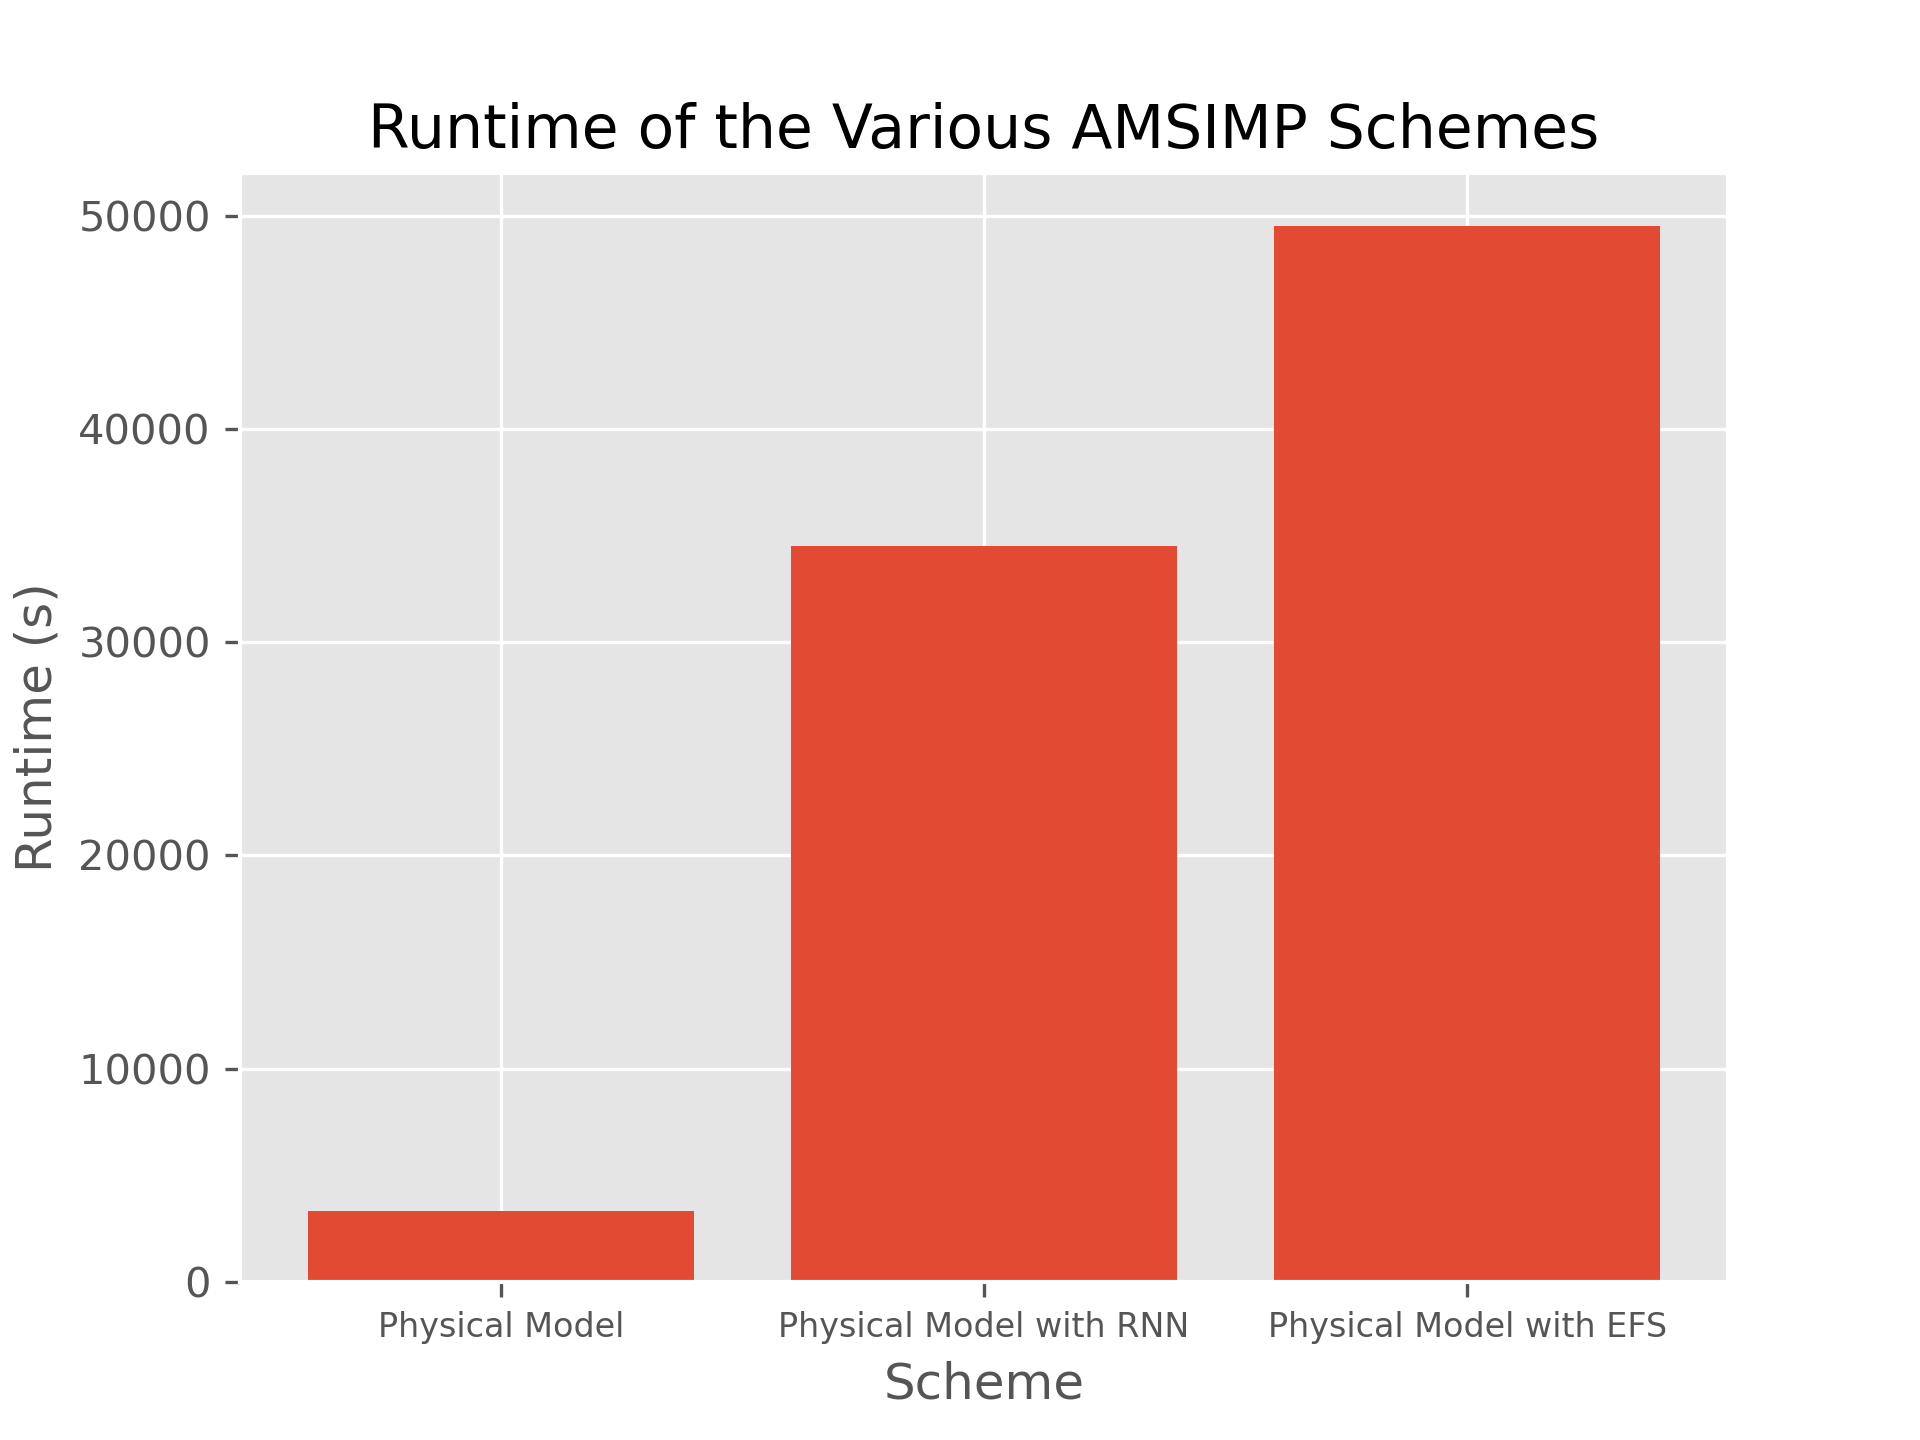
\includegraphics[width=.8\linewidth]{Graphs/performance/runtime.png}
    \caption{Runtime of Various AMSIMP Schemes}
\end{figure}

\begin{figure}[H]
    \centering
    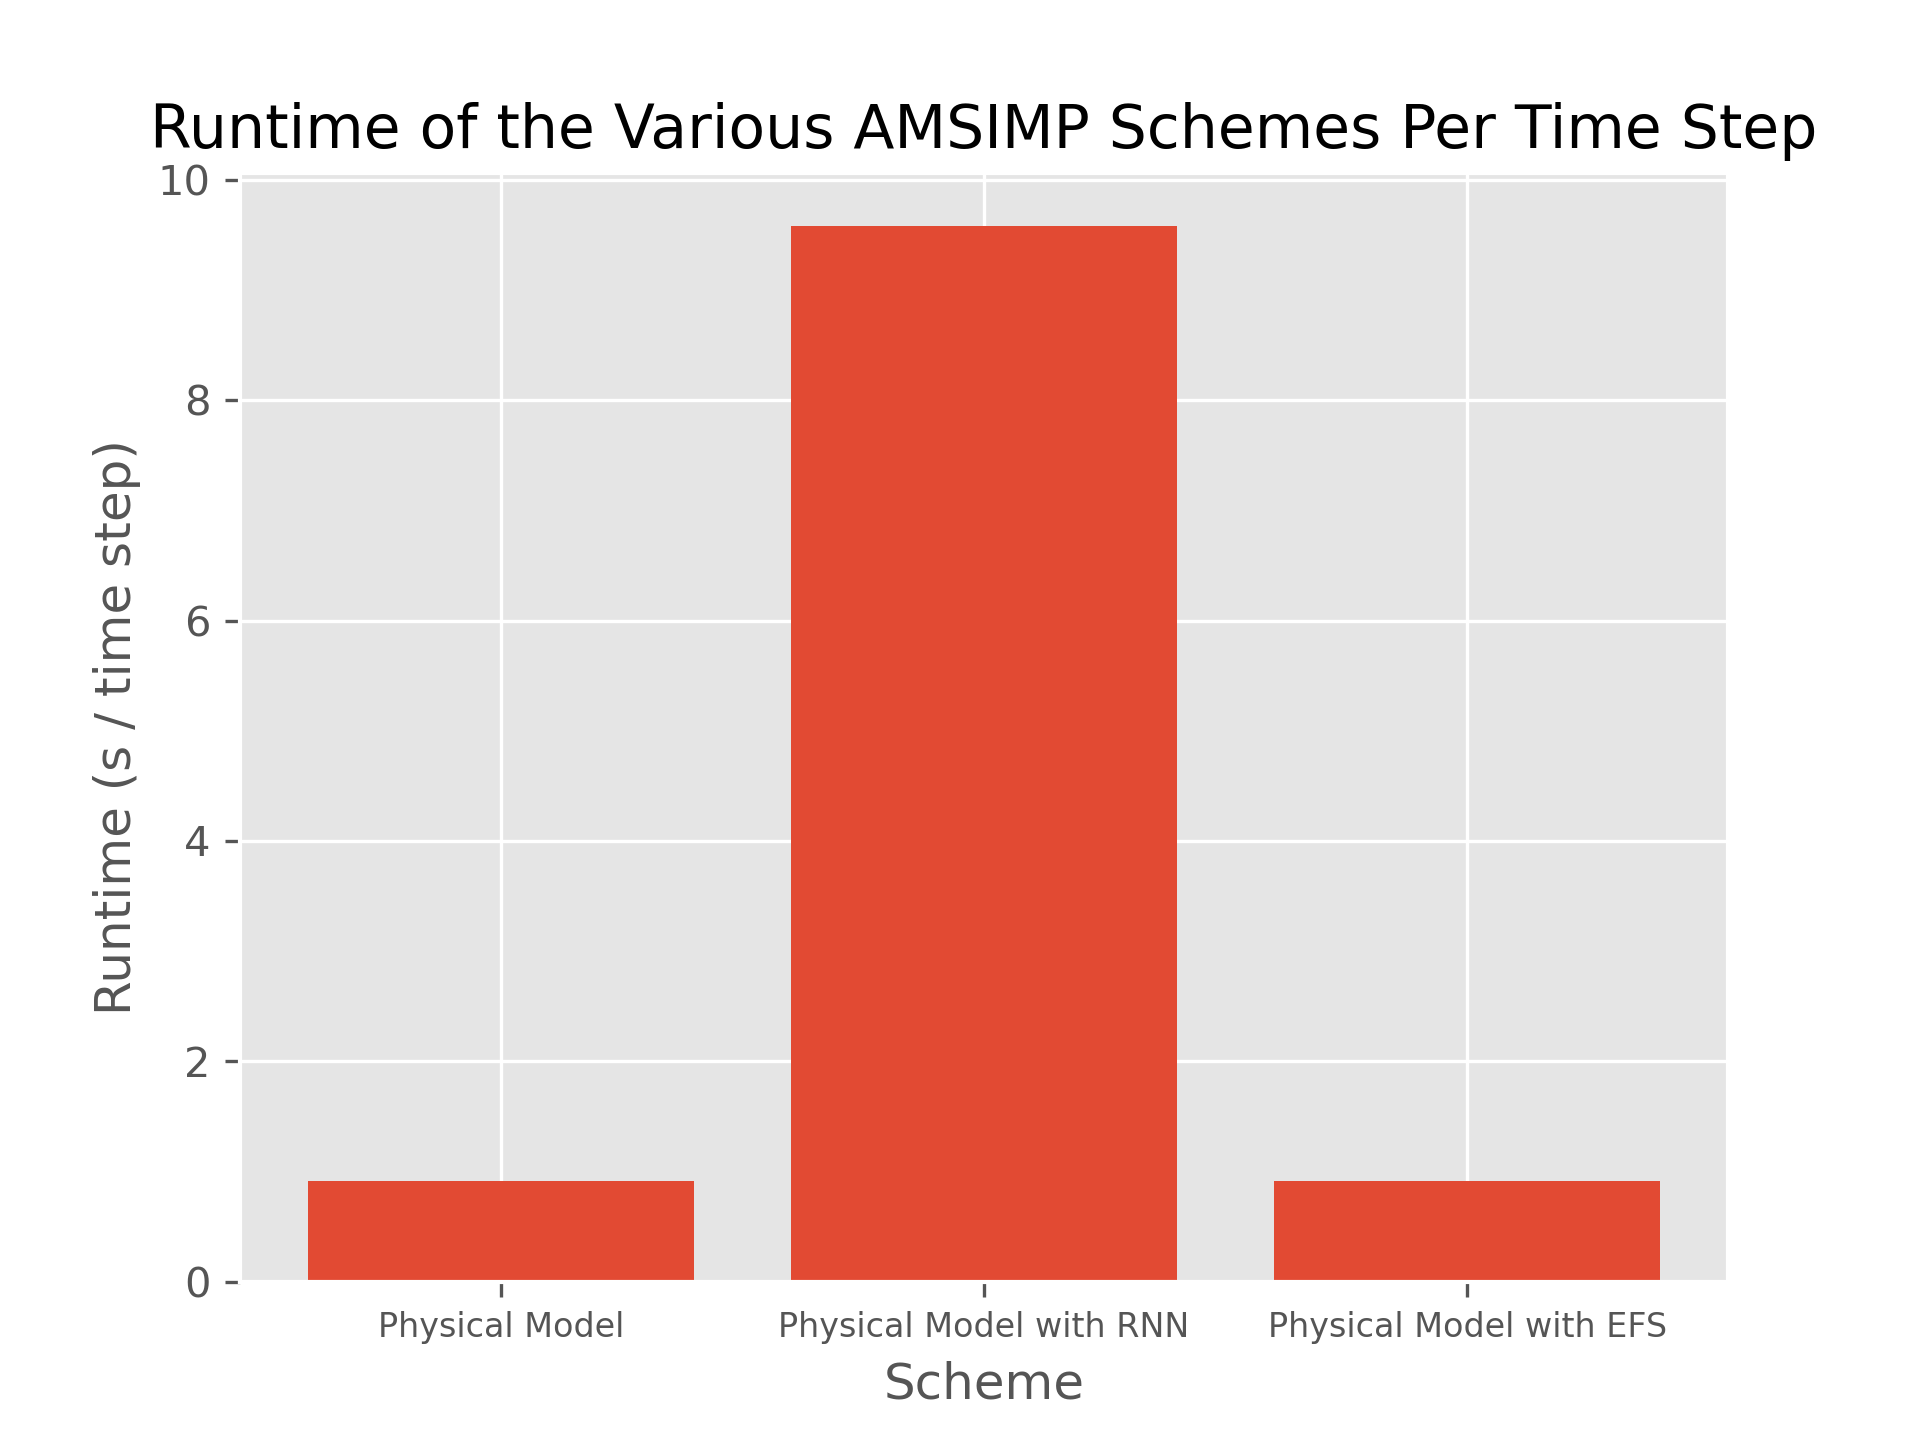
\includegraphics[width=.8\linewidth]{Graphs/performance/runtime_per_timestep.png}
    \caption{Runtime of Various AMSIMP Schemes Per Time Step}
\end{figure}

\begin{figure}[H]
    \centering
    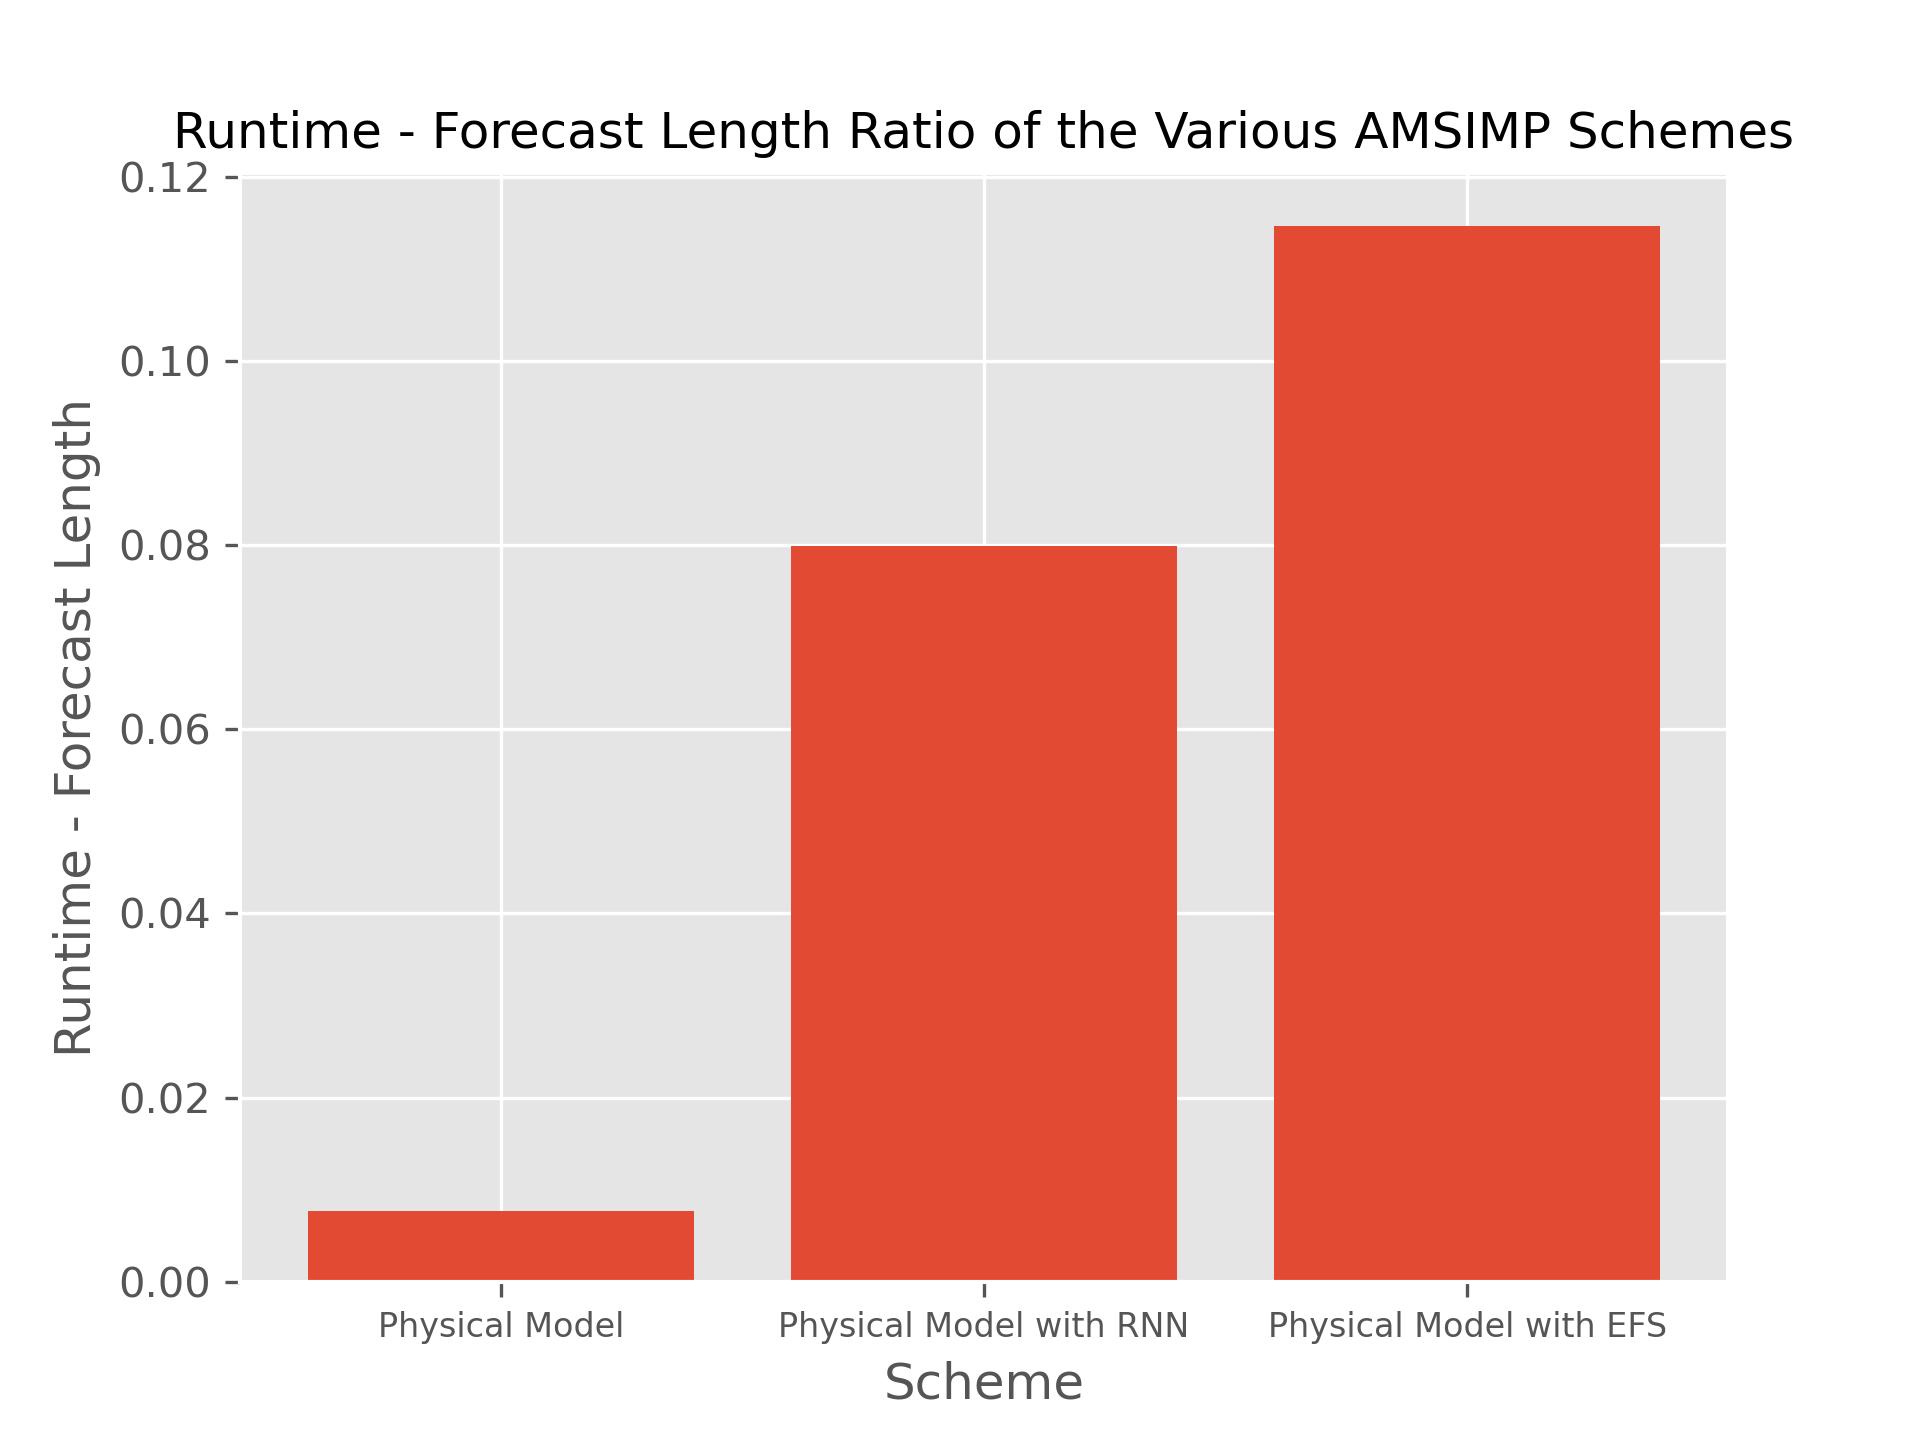
\includegraphics[width=.8\linewidth]{Graphs/performance/ratio.png}
    \caption{Runtime - Forecast Length Ratio of the Various AMSIMP Schemes}
\end{figure}

\section{Accuracy Benchmark}
\subsection{Mean Absolute Scaled Error}
\begin{figure}[H]
    \centering
    \includegraphics[width=.7\linewidth]{Graphs/accuracy/mase/temperature.png}
    \caption{AMSIMP Air Temperature Mean Absolute Scaled Error}
\end{figure}

\begin{figure}[H]
    \centering
    \includegraphics[width=.7\linewidth]{Graphs/accuracy/mase/virtual_temperature.png}
    \caption{AMSIMP Virtual Temperature Mean Absolute Scaled Error}
\end{figure}

\begin{figure}[H]
    \centering
    \includegraphics[width=.8\linewidth]{Graphs/accuracy/mase/relative_humidity.png}
    \caption{AMSIMP Relative Humidity Mean Absolute Scaled Error}
\end{figure}

\begin{figure}[H]
    \centering
    \includegraphics[width=.8\linewidth]{Graphs/accuracy/mase/geopotential_height.png}
    \caption{AMSIMP Geopotential Height Mean Absolute Scaled Error}
\end{figure}

\begin{figure}[H]
    \centering
    \includegraphics[width=.8\linewidth]{Graphs/accuracy/mase/zonal_wind.png}
    \caption{AMSIMP Zonal Wind Mean Absolute Scaled Error}
\end{figure}

\begin{figure}[H]
    \centering
    \includegraphics[width=.8\linewidth]{Graphs/accuracy/mase/meridional_wind.png}
    \caption{AMSIMP Meridional Wind Mean Absolute Scaled Error}
\end{figure}

\subsection{Comparison of Schemes}
\begin{figure}[H]
    \centering
    \includegraphics[width=.8\linewidth]{Graphs/accuracy/comparsion_schemes/temperature.png}
    \caption{AMSIMP Air Temperature Mean Squared Error}
\end{figure}

\begin{figure}[H]
    \centering
    \includegraphics[width=.8\linewidth]{Graphs/accuracy/comparsion_schemes/virtual_temperature.png}
    \caption{AMSIMP Virtual Temperature Mean Squared Error}
\end{figure}

\begin{figure}[H]
    \centering
    \includegraphics[width=.8\linewidth]{Graphs/accuracy/comparsion_schemes/relative_humidity.png}
    \caption{AMSIMP Relative Humidity Mean Squared Error}
\end{figure}

\begin{figure}[H]
    \centering
    \includegraphics[width=.8\linewidth]{Graphs/accuracy/comparsion_schemes/geopotential_height.png}
    \caption{AMSIMP Geopotential Height Mean Squared Error}
\end{figure}

\begin{figure}[H]
    \centering
    \includegraphics[width=.8\linewidth]{Graphs/accuracy/comparsion_schemes/zonal_wind.png}
    \caption{AMSIMP Zonal Wind Mean Squared Error}
\end{figure}

\begin{figure}[H]
    \centering
    \includegraphics[width=.8\linewidth]{Graphs/accuracy/comparsion_schemes/meridional_wind.png}
    \caption{AMSIMP Meridional Wind Mean Squared Error}
\end{figure}

\subsection{Comparison against OpenWeatherAPI}
\begin{figure}[H]
    \centering
    \includegraphics[width=.8\linewidth]{Graphs/accuracy/comparsion_openweatherapi/temperature.png}
    \caption{Air Temperature Mean Squared Error}
\end{figure}

\begin{figure}[H]
    \centering
    \includegraphics[width=.8\linewidth]{Graphs/accuracy/comparsion_openweatherapi/virtual_temperature.png}
    \caption{Virtual Temperature Mean Squared Error}
\end{figure}

\begin{figure}[H]
    \centering
    \includegraphics[width=.8\linewidth]{Graphs/accuracy/comparsion_openweatherapi/relative_humidity.png}
    \caption{Relative Humidity Mean Squared Error}
\end{figure}

\begin{figure}[H]
    \centering
    \includegraphics[width=.8\linewidth]{Graphs/accuracy/comparsion_openweatherapi/zonal_wind.png}
    \caption{Zonal Wind Mean Squared Error}
\end{figure}

\begin{figure}[H]
    \centering
    \includegraphics[width=.8\linewidth]{Graphs/accuracy/comparsion_openweatherapi/meridional_wind.png}
    \caption{Meridional Wind Mean Squared Error}
\end{figure}

\chapter{Conclusions}\label{conclusion_chapter}
\epigraph{``It is our choices, Harry, that show what we truly are, far more than our abilities."}{Albus Dumbledore}

The previous chapters have discussed the development of an open source implementation to improve numerical weather prediction through the utilisation of a neural network architecture. Although extremely time consuming, the importance of an open source implementation cannot be understated. It could potentially open up a field to a wider group, and often doesn't receive the media attention it rightfully deserves. 

Future applications of this work are extremely wide ranging, from usage in numerical weather prediction schemes that take in observational data collected from satellites, and ground stations in order to provide a picture of future weather events; to forming a starting point in future research of atmospheric phenomena. While, at the moment, it definitely would be inaccurate to say the software is ready for such usage, with future enhancements which I will touch on in a minute, it most certainly will.

\section{Looking Back}
To prove the hypothesis that `it is possible to train a neural network on an atmospheric reanalysis dataset based on data from the 10 years, that such a neural network captures crucial weather patterns, and can predict the future evolution of the atmosphere, and that such a machine learning model will ultimately improve numerical weather prediction in comparison to established physics-based models.', it was necessary to carry out a series of appropriate benchmarks.

\subsection{Analysis of Results}
This report hypothesises that it is possible to train a neural network on an atmospheric reanalysis dataset based on data from the 10 years, that such a neural network captures crucial weather patterns, and can predict the future evolution of the atmosphere, and that such a machine learning model will ultimately improve numerical weather prediction in comparison to established physics-based models.

To gain an insight into the future feasibility of neural networks in the field of meteorology, a comparison between the performance of the current model against the performance of the previous LSTM model is shown in section \ref{old_model}. Air temperature is the only parameter examined for this comparison, as the previous model did not incorporate geopotential. Concerning the two metrics, root mean squared error and mean absolute error, there has been a dramatic performance improvement. There has been a mean decrease of 52.5 \% in the root mean squared error values, and a mean decrease of 48.6 \% in the mean absolute error values; on average a 50.6 \% decrease in error metrics across the board. This demonstrates the continued improvement and enhancement of the models over the last few months; but, it also demonstrates that the performance of the software can still be improved drastically. The performance increase has not reached a plateau, which is extremely promising.

One of the key factors which led to the development of a machine learning model was the expected decrease in computational resources required to generate a forecast. While the initial training of the model was computationally burdensome, particularly with respect to memory, the assumption made at the start of this project holds once the model is trained. Once the model has trained, a performance increase of 6.18 times can be expected in comparison against a physics-based model of a similar resolution, the ECMWF IFS T63. It is also important to note that the benchmark of the software was run on a consumer-grade, MacBook Pro while the benchmark of the ECMWF IFS T63 model was performed on a single XC40 node with 36 cores. Hence, a further increase in performance can be expected with a similar configuration.

With respect to the benchmarking outlined in chapter \ref{benchmarking_chapter}, the forecast system needs to beat the climatology forecast and the persistence forecast to be classified as useful. The benchmarks have demonstrated that the model can be generally regarded as useful, particularly on longer periods and in relation to air temperature, in particular, however, the models generally fail to beat well established physics-based models at this time. The model is significantly better at creating air temperature predictions and appears to suffer with geopotential predictions. The root mean squared error and mean squared error demonstrate that the model's air temperature becomes useful after approximately 24 hours of forecast time, with the model ultimately beating the ECMWF IFS T42 model after approximately 96 hours. The picture for geopotential is less rosy, with the root mean squared error and mean squared error demonstrating that the model's geopotential predictions become useful after approximately 96 hours of forecast time. An interesting point to note is that the error values initially are quite high, the error values appear to plateau. This may suggest that the model may be quite useful at generating climate forecasts. Concerning spatial awareness as measured by the anomaly correlation coefficient, both the mode's geopotential and air temperature predictions become useful after approximately 120 hours of forecast time. The spatial awareness of the model can be generally regarded as quite poor, it appears that the spatial aspect of a weather forecast was not captured by the model. 

Hence, the hypothesis that was proposed has partially been proven and can be accepted, as such.

\subsection{Sources of Error}

Hence, the hypothesis that was proposed has partially been proven, however, there are a few areas which could have hindered the performance of the software or led to a possible source of error:

\begin{itemize}
    \item As mentioned in section \ref{era5_dataset}, it was decided to use a spatial resolution of $1^{\circ}$ ($179 \times 360$ grid points) and a temporal resolution of 2 hours. A lower resolution was chosen in order to reduce the amount of computational resources required to train the model. Through high spatial resolution, however, a forecast can show the effects of local air currents, topography and soil cover. The forecasts produced thereby show local weather differences in more precise way\cite{res}. High resolution produces high precision, hence, while choosing a lower resolution may have lowered the computational burden during training, it may have had a significant on the performance of the model.
\end{itemize}

\section{Looking Ahead}
The software is currently in an alpha release state. An alpha version of any software is a very early version of the software that may not contain all of the features that are planned for the final version\cite{alpha}. In this section, I will briefly outline the enhancements and features that will be released in the beta version of the software, which is planned for release in Spring 2021:

\begin{itemize}
    \item One of the most natural coordinate systems to use on Earth is a latitude‐longitude grid. This was the coordinate system of choice for this project due to its simplicity, but, this system has singularities at the North Pole and South Pole that makes it difficult to use translationally‐invariant convolution operations on this grid. To combat this particular problem in this project, the poles were excluded from the dataset, however, a more elegant solution to preserve spatial locality is to approximate data on the globe using the cubed sphere. This projection has been shown to give more uniformly sized grid cells than the alternative projections and to also produce better solutions to finite‐difference and discontinuous Galerkin approximations to partial differential equations on the sphere. The cubed sphere is used for state‐of‐the‐art NWP such as in the FV3 dynamical core of the National Oceanic and Atmospheric Administration's Global Forecast System model\cite{cubed_sphere}. This is an avenue that will be explored in the coming months. 
    \item As mentioned previously, a high resolution weather forecast produces high precision. As a result, in order to improve the performance of the model, the model will be trained on a higher resolution dataset. At this point, a resolution has not been decided, however, the decision will be made based on the computational resources available to initially train the model and the expected increase in performance that could be made by switching to a higher resolution. 
    \item The three parameters on which the machine learning models were trained upon were: air temperature at 850 hPa, geopotential at 500 hPa, and air temperature at 2 metres above the surface. While these parameters are extremely important to predict from a meteorological point of view, the general public require predictions for the amount of precipitation to be made several days in advance; in order to make personal, and business decisions. This may be supplying shops with more food during periods of snowfall, or county councils setting up flood defences in town. In the coming months, the model will be trained on such parameters in order to provide the most useful weather forecast possible.  
\end{itemize}

\newpage

\appendix
\renewcommand{\thesection}{\Alph{section}.\arabic{section}}
\setcounter{section}{0}
\begin{appendices}
    \section{Code for the AMSIMP Global Forecast Model}\label{model_code}
    \begin{minted}[mathescape,linenos,frame=lines]{python}
def model(epochs, bs):
    # Number of elements.
    n = len(os.listdir("processed_dataset/"))
    lst_n = np.linspace(1, n, n)
    
    # Define training dataset and validation dataset.
    # Training.
    train_ns = lst_n[:int(0.7 * n)]
    train_generator = DataGenerator(
        train_ns,
        batch_size=bs,
    )
    print("Training dataset created.")
    
    # Validation.
    val_ns = lst_n[int(0.7 * n):int(0.9 * n)]
    val_generator = DataGenerator(
        val_ns, 
        batch_size=bs,
        shuffle=False
    )
    print("Validation dataset created.")
    
    with mirrored_strategy.scope():
        # Create, and train models.
        # Optimiser.
        opt = Adam(lr=1e-3, decay=1e-5)
        # Create model.
        model = Sequential()

        # First layer.
        model.add(
            ConvLSTM2D(
                filters=64, 
                kernel_size=(7, 7),
                input_shape=(6, 179, 360, 3), 
                padding='same', 
                return_sequences=True, 
                activation='tanh', 
                recurrent_activation='hard_sigmoid',
                kernel_initializer='glorot_uniform', 
                unit_forget_bias=True, 
                dropout=0.3, 
                recurrent_dropout=0.3, 
                go_backwards=True
            )
        )
        # Batch normalisation.
        model.add(BatchNormalization())
        # Dropout.
        model.add(Dropout(0.1))
        
        # Second layer.
        model.add(
            ConvLSTM2D(
                filters=32, 
                kernel_size=(7, 7), 
                padding='same', 
                return_sequences=True, 
                activation='tanh', 
                recurrent_activation='hard_sigmoid', 
                kernel_initializer='glorot_uniform', 
                unit_forget_bias=True, 
                dropout=0.4, 
                recurrent_dropout=0.3, 
                go_backwards=True
            )
        )
        # Batch normalisation.
        model.add(BatchNormalization())
        
        # Third layer.
        model.add(
            ConvLSTM2D(
                filters=32, 
                kernel_size=(7, 7), 
                padding='same', 
                return_sequences=True, 
                activation='tanh', 
                recurrent_activation='hard_sigmoid', 
                kernel_initializer='glorot_uniform', 
                unit_forget_bias=True, 
                dropout=0.4, 
                recurrent_dropout=0.3, 
                go_backwards=True
            )
        )
        # Batch normalisation.
        model.add(BatchNormalization())
        # Dropout.
        model.add(Dropout(0.1))

        # Final layer.
        model.add(
            ConvLSTM2D(
                filters=32, 
                kernel_size=(7, 7), 
                padding='same', 
                return_sequences=True, 
                activation='tanh', 
                recurrent_activation='hard_sigmoid', 
                kernel_initializer='glorot_uniform', 
                unit_forget_bias=True, 
                dropout=0.5, 
                recurrent_dropout=0.3, 
                go_backwards=True
            )
        )
        # Batch normalisation.
        model.add(BatchNormalization())

        # Add dense layer.
        model.add(Dense(3))
    
    # Compile model.
    model.compile(
        optimizer=opt, 
        loss='mse'
    )
    # Summary of model.
    model.summary()

    # Train.
    model.fit(
        train_generator,
        validation_data=val_generator,
        epochs=epochs,
        callbacks=[
            tf.keras.callbacks.EarlyStopping(
                monitor="val_loss", min_delta=0, patience=2, mode="auto"
            )
        ],
    )
    
    return model
    \end{minted}
    
    \section{Comparison against Previous Model}\label{old_model}
    \begin{figure}[H]
        \centering
        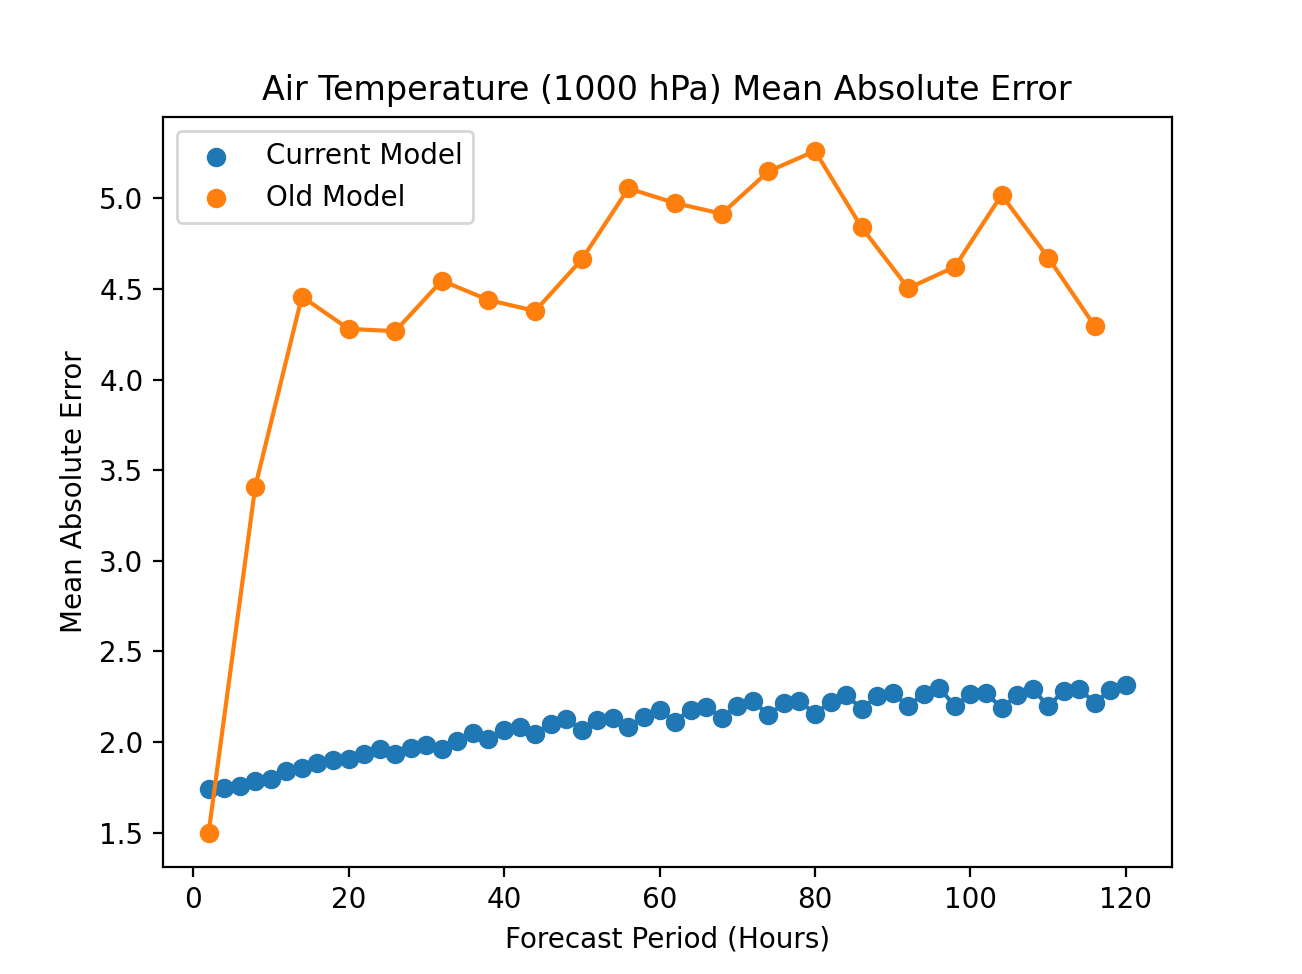
\includegraphics[width=.7\linewidth]{Plots/Results/Temperature/t1000_mae.png}
        \caption{MAE for Air Temperature at 1000 hPa}
    \end{figure}
    
    \begin{figure}[H]
        \centering
        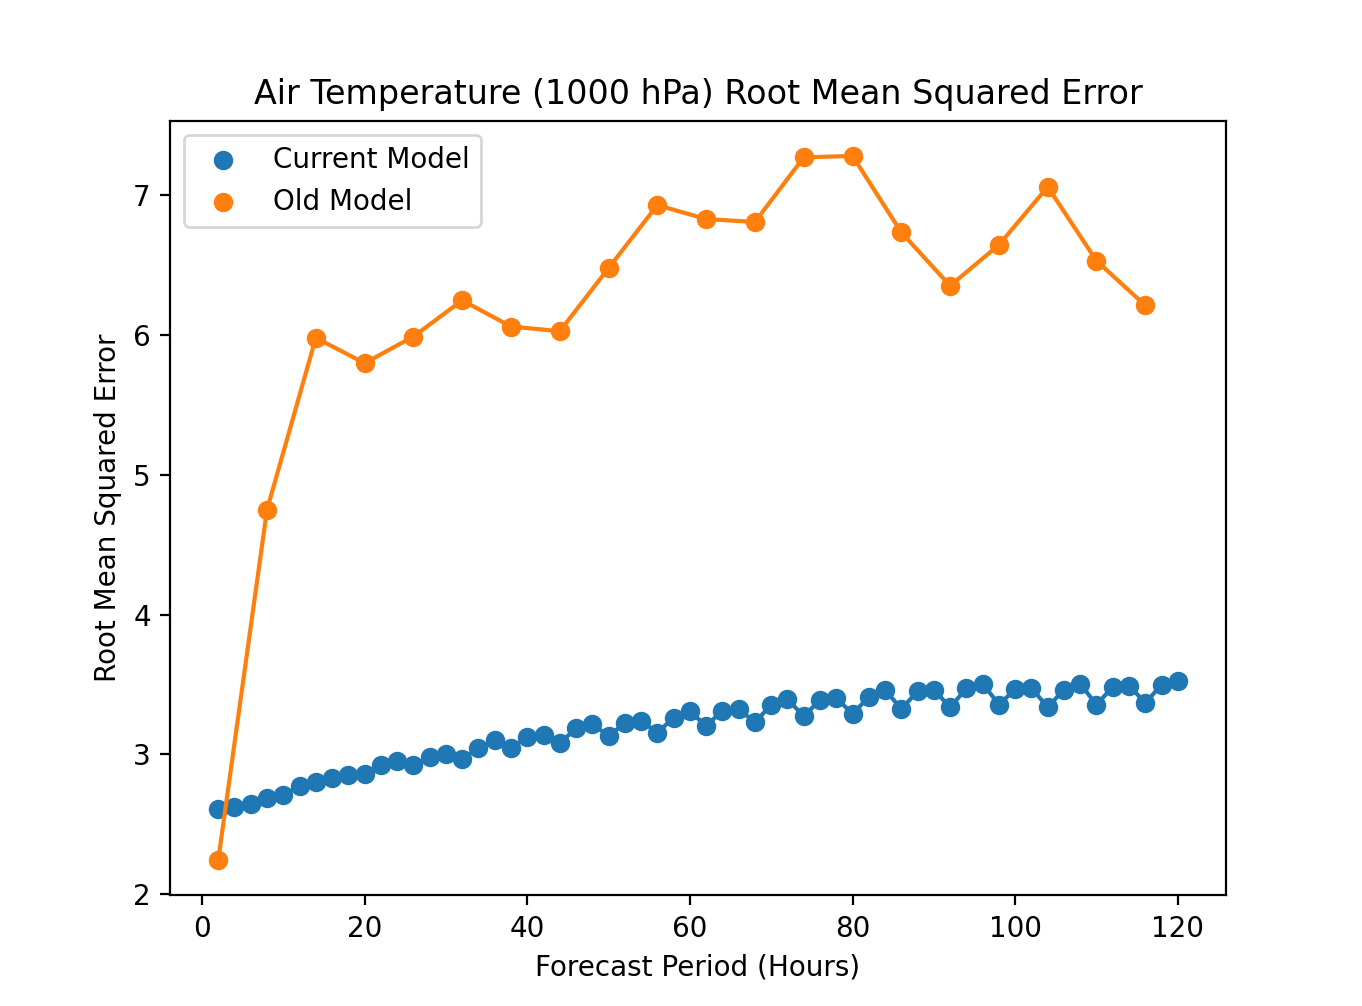
\includegraphics[width=.7\linewidth]{Plots/Results/Temperature/t1000_rmse.png}
        \caption{RMSE for Air Temperature at 1000 hPa}
    \end{figure}
\end{appendices}

\printbibliography[heading = bibintoc]

\end{document}